


\section{Related Work}

\subsection{Generalist Game Agents}

Research on game-playing agents has expanded from environment-specific policies to general models combining perception, reasoning, memory, and executable control. Large-scale behavioral pretraining provides one route: VPT~\cite{baker2022vpt} learns Minecraft control from internet videos labeled by an inverse dynamics model, while STEVE-1~\cite{lifshitz2023steve1} extends this paradigm to language-conditioned behavior. Other systems, including DEPS~\cite{wang2023deps}, Voyager~\cite{wang2023voyager}, JARVIS-1~\cite{wang2025jarvis1}, Optimus-1~\cite{li2024optimus1}, and OmniJARVIS~\cite{wang2024omnijarvis}, incorporate planning, reusable skills, and memory to support increasingly complex tasks. 

Recent work further targets generalization across tasks and worlds. Gato~\cite{reed2022gato} and SIMA~\cite{simateam2024sima} study shared policies across heterogeneous environments, while Game-TARS~\cite{wang2025gametars} and Lumine~\cite{tan2025lumine} combine reasoning, memory, and native keyboard–mouse control for extended gameplay. NitroGen~\cite{magne2026nitrogen} and OpenP2P ~\cite{yue2026openp2p} instead emphasize scalable visual policy learning from broad gameplay data. These approaches address different aspects of generalist gameplay, typically emphasizing cross-environment reactive control or extended reasoning under more specialized training settings. We combine cross-game continued pre-training with task-oriented policy optimization for sustained interaction.

\subsection{Scalable Gameplay Learning}

Progress in game agents increasingly relies on large and heterogeneous interaction data. MineRL~\cite{guss2019minerl} and MineDojo~\cite{fan2022minedojo} provide structured demonstrations and multimodal resources, while VPT~\cite{baker2022vpt} scales behavioral learning through inverse dynamics. D2E~\cite{choi2026d2e}, NitroGen~\cite{magne2026nitrogen}, and OpenP2P~\cite{yue2026openp2p} broaden supervision through desktop trajectories, visible control overlays, and inverse-dynamics-labeled gameplay. GameHorizon~\cite{wang2026gamehorizon} further introduces multi-level annotations spanning operations, subgoals, and strategies. 

Transfer also depends on model size and data composition. General scaling and continual-pretraining studies show that performance depends jointly on model capacity, data budget, and domain mixture. In gameplay, VPT~\cite{baker2022vpt} demonstrates the value of large-scale behavioral pretraining, while OpenP2P~\cite{yue2026openp2p} studies scaling through both predictive performance and causal behavior. GameScaling varies model size, interaction budget, and game composition to distinguish between gains obtained by learning a shared control interface and gains that depend on target-relevant gameplay. Scale alone is not sufficient for task-oriented gameplay. Effective policy learning also requires supervision that connects local actions with higher-level objectives. GameHorizon~\cite{wang2026gamehorizon} introduces temporal hierarchy into gameplay supervision, while OmniJARVIS~\cite{wang2024omnijarvis} and Lumine~\cite{tan2025lumine} combine reasoning, memory, and staged training. We train the policy with supervision at the operation, subgoal, and task levels, and retain compact task summaries across context boundaries.


\subsection{Memory and Long-Horizon Interaction}

Sustained gameplay also requires agents to retain task-relevant information after earlier interactions leave the active context. Existing agents address this through reusable skills, retrieved experience, or compressed interaction histories. Voyager stores executable skills, JARVIS-1~\cite{wang2025jarvis1} and Optimus-1~\cite{li2024optimus1} retrieve accumulated experience, and Game-TARS~\cite{wang2025gametars} combines recent interactions with compressed textual history. OmniJARVIS~\cite{wang2024omnijarvis} and Lumine~\cite{tan2025lumine} further integrate memory with reasoning and action generation. We explicitly supervise task summaries and use them as persistent task state during supervised training, online policy optimization, and streaming inference. 

Feedback-based optimization provides a complementary mechanism for improving extended behavior. GRPO~\cite{shao2024deepseekmath} optimizes relative advantages across groups of sampled outputs, while GUI-R1~\cite{luo2025gui} and Game-RL~\cite{tong2026gamerl} adapt reinforcement learning to executable GUI actions and multimodal game reasoning. Game-TARS~\cite{wang2025gametars} also refines thought–action trajectories through action-consistency-based filtering. We optimize finite trajectory segments linked by compressed memory, updating task-state maintenance and executable behavior together. Long-horizon interaction must also operate under bounded context and latency. StreamingLLM~\cite{xiao2024streamingllm} maintains stable inference with a fixed attention window, while InfiniPot-V~\cite{kim2025infinipotv}, DSCache~\cite{pang2026dscache}, and StreamingVLM~\cite{xu2026streamingvlm} explore compressed or structured memory for continuous visual streams. Serving techniques such as PagedAttention~\cite{kwon2023pagedattention} and speculative decoding further reduce autoregressive inference cost. These directions are largely studied separately from long-horizon policy optimization. Our streaming engine uses bounded memory, cache reuse, and the task representation learned during training to sustain interaction within context and latency limits.

\ourmodel combines cross-game behavioral scaling, multi-level task supervision, and memory-supported long-horizon interaction in one policy.

\section{CPT Scaling and Cross-Game Generalization}
\label{app:cpt_scaling}
\subsection{Data Mixtures and Validation Distributions}
\label{app:cpt_diversity}

The controlled CPT grid holds its source inventory fixed while varying the share of Minecraft trajectories. S1 uses Minecraft exclusively. S2-S4 draw from the same 80 canonical game labels with different sampling weights, and S5 removes Minecraft, leaving 79 labels. You can find more details in Table~\ref{tab:cpt_mixture_diversity}. Consequently, the five mixtures should not be interpreted as a monotonic increase in the number of game worlds. We summarize diversity using the effective number of worlds, $\exp(-\sum_w p_w\log p_w)$, which accounts for the balance of gameplay samples across game labels.

\begin{table}[t]
\centering\small
\caption{\textbf{Measured diversity of the CPT game mixtures.} World labels are canonicalized across sources. Effective worlds denotes exponential Shannon diversity, while the inverse Simpson index emphasizes high-probability worlds.}
\label{tab:cpt_mixture_diversity}
\setlength{\tabcolsep}{4pt}
\begin{tabular}{lrrrrr}
\toprule
Mixture & Worlds & MC share & Largest share & Eff. worlds & Inv. Simpson\\
\midrule
S1 & 1 & 100.0\% & 100.0\% & 1.0 & 1.0\\
S2 & 80 & 51.4\% & 51.4\% & 14.5 & 3.7\\
S3 & 80 & 27.1\% & 27.1\% & 35.2 & 11.9\\
S4 & 80 & 2.8\% & 4.2\% & 60.1 & 52.6\\
S5 & 79 & 0.0\% & 4.3\% & 58.7 & 51.0\\
\bottomrule
\end{tabular}
\end{table}

The fixed non-Minecraft pool contains 124 source-stream labels mapping to 79 canonical game labels. The three validation distributions separate Minecraft held-out clips, training-covered game clips, and title-disjoint unseen-game clips. The latter is game-balanced, with 28 unseen titles and 160 clips per title (4,480 clips in total). Grouping by source recording and removing title aliases limit overlap between training and validation. These splits distinguish transfer of the action interface from gains limited to games in the training mixture.

\subsection{Scaling Results from GameScaling}
\label{app:gamescaling_results}

This subsection collects the scaling results from GameScaling~\cite{gamescaling} summarized in Sec.~\ref{sec:exp_cpt_scaling}. These results characterize how model size, gameplay budget, and game composition affect CPT within the evaluated configurations and provide context for Gamer's CPT stage.

\begin{figure*}[!htbp]
    \centering
    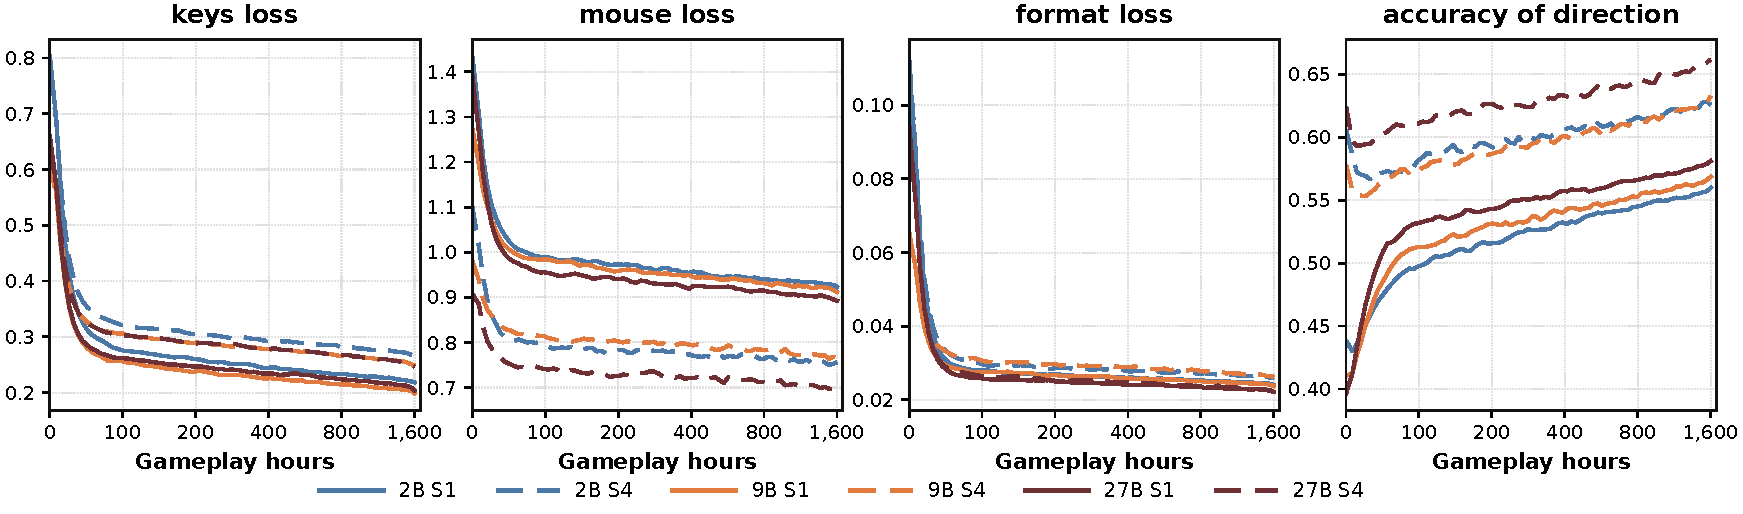
\includegraphics[width=0.85\linewidth]{figs/cpt-action-losses.pdf}
    \caption{
    \textbf{Early adaptation to the shared keyboard-mouse interface.}
    The figure reports keyboard, mouse, and action-format losses together with directional prediction accuracy for 2B, 9B, and 27B models under the S1 and S4 mixtures.
    The horizontal axis denotes cumulative gameplay hours. Results from GameScaling~\cite{gamescaling}.
    }
    \label{fig:cpt_action_losses}
\end{figure*}

\paragraph{Interface adaptation.}
Figure~\ref{fig:cpt_action_losses} reports keyboard, mouse, and action-format losses together with directional prediction accuracy. The rapid early decrease in these losses and the improvement in directional accuracy suggest that initial CPT learning partly concerns adaptation to the shared keyboard-mouse interface.

\begin{figure*}[!t]
    \centering
    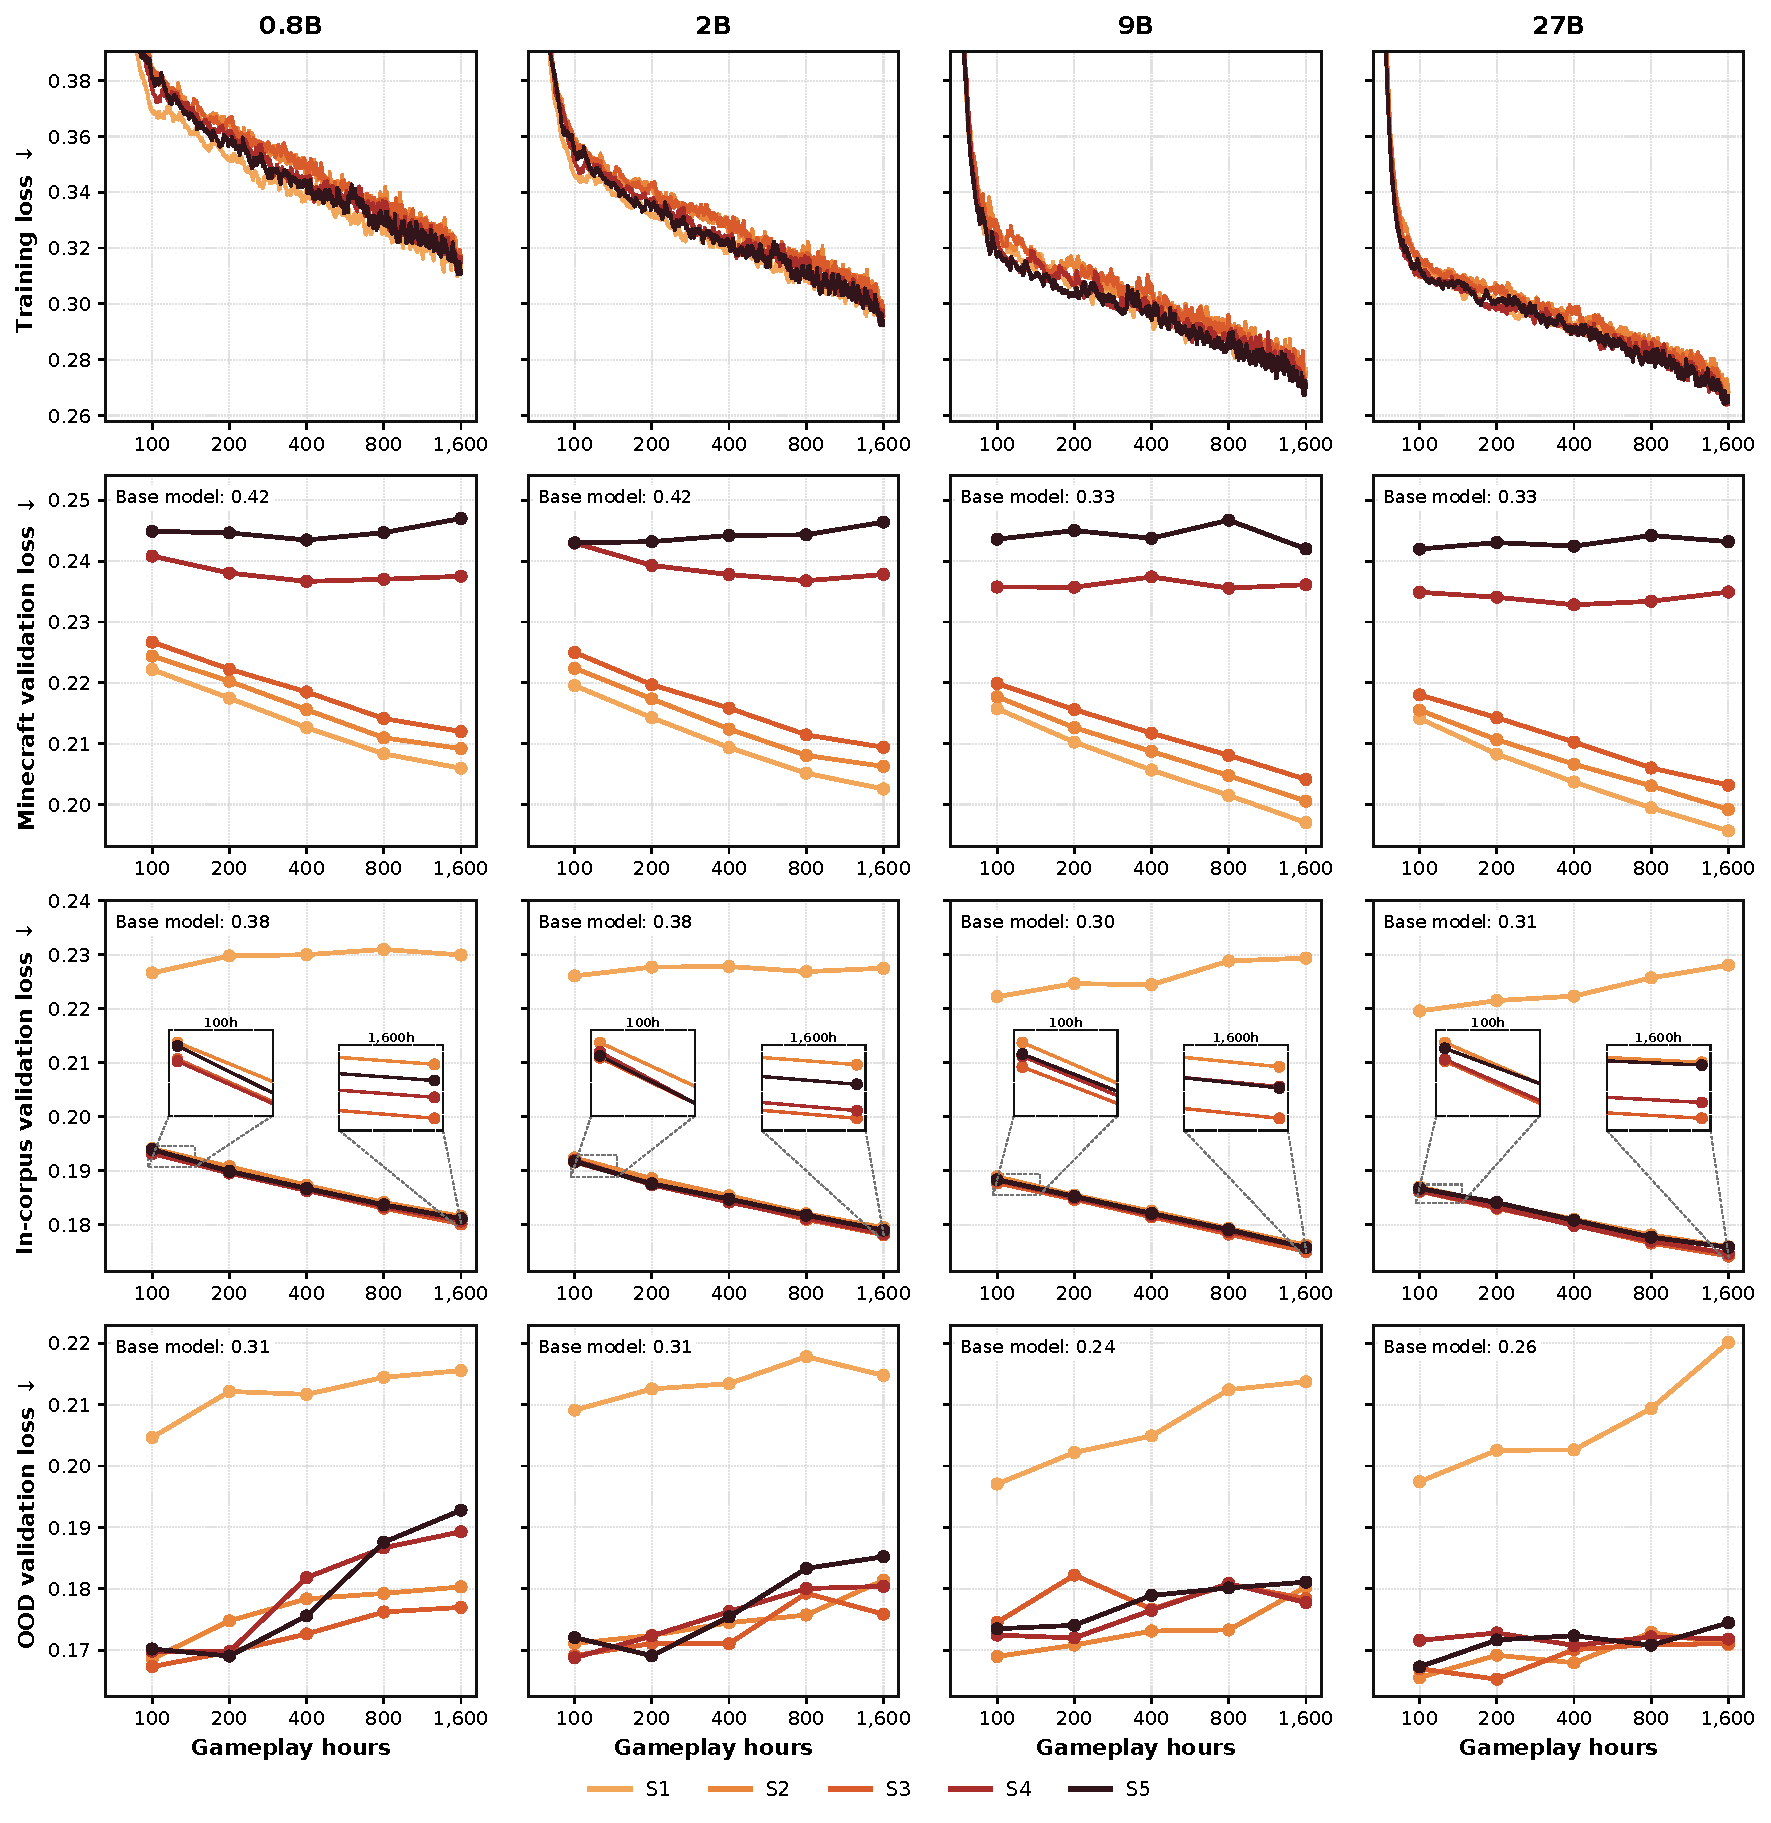
\includegraphics[width=0.83\linewidth]{figs/cpt-scaling-losses.pdf}
    \caption{
    \textbf{CPT scaling depends on model capacity, interaction budget, and game composition.}
    The rows show training loss, Minecraft validation loss, validation loss on other training games, and validation loss on unseen games.
    Columns correspond to model scale, while S1-S5 denote different game mixtures.
    The final column compares fitted and measured losses. Results from GameScaling~\cite{gamescaling}.
    }
    \label{fig:cpt_scaling_losses}
\end{figure*}

\paragraph{Training and validation losses.}
Figure~\ref{fig:cpt_scaling_losses} reports training loss and validation losses on Minecraft, other training games, and unseen games. The curves show that gains from additional gameplay data depend on model capacity and game composition. In particular, validation loss on distant unseen games plateaus or increases after early adaptation, even while training loss continues to decrease.

\begin{figure*}[!t]
    \centering
    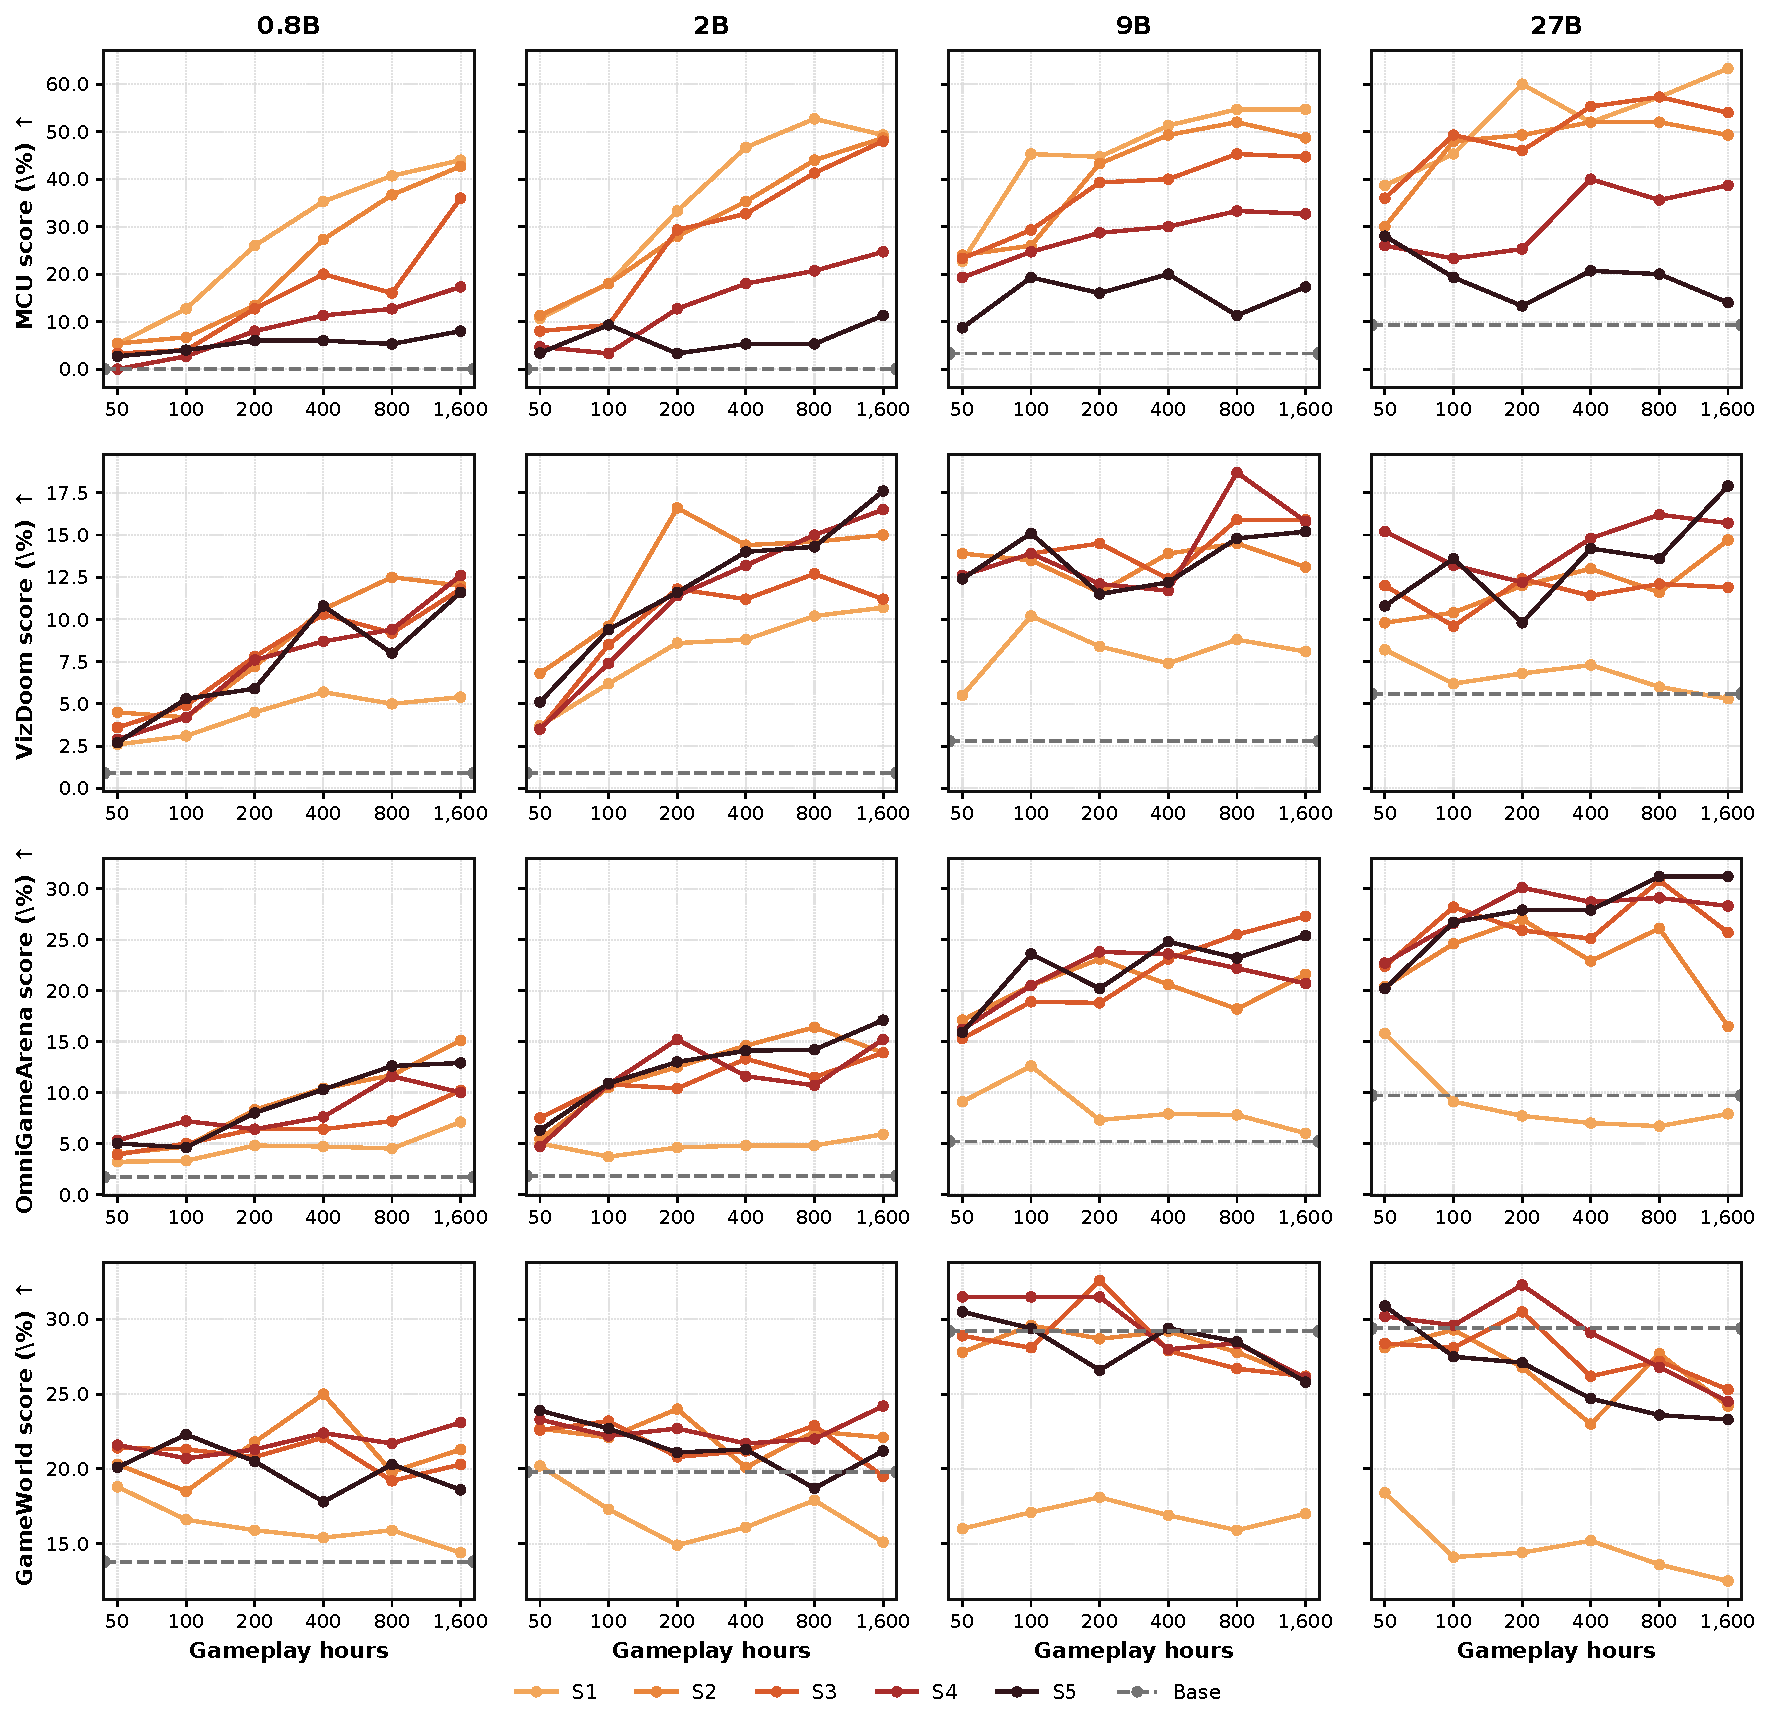
\includegraphics[width=0.77\linewidth]{figs/gamescaling_benchmark_hours.pdf}
    \caption{\textbf{Gameplay benchmark scaling across training budgets.} Rows show MCU, ViZDoom, OmniGameArena, and GameWorld, and columns show the four Qwen3.5 Dense scales. Colored curves compare the S1-S5 training mixtures across 50-1,600 gameplay hours, with dashed lines denoting the unadapted backbone. Multi-game mixtures support transfer to related environments. Scores are measured under time-paused interaction. Results from GameScaling~\cite{gamescaling}.}
    \label{fig:cpt_benchmark_hours}
\end{figure*}

\paragraph{Gameplay benchmark performance.}
Figure~\ref{fig:cpt_benchmark_hours} reports performance on MCU, ViZDoom, OmniGameArena, and GameWorld under time-paused interaction. These results complement the validation-loss analysis with executable gameplay outcomes. Within the evaluated configurations, mixed-game training supports transfer to related environments, while gains on more distant games remain limited.

\subsection{Composition-Aware Scaling-Law Fitting}
\label{app:cpt_scaling_fit}

This subsection summarizes the fitting procedure and results reported in GameScaling~\cite{gamescaling}, using the notation of Sec.~\ref{sec:cpt_scaling}.
The composition-aware scaling relation is fitted separately to Minecraft validation loss and validation loss over the remaining training-game distribution:
\begin{equation}
\mathcal{L}_{\mathrm{val}}(N,D,q)
=
E
+
\frac{C_N}{N^a}
+
\frac{C_D q^\eta}{D^b}
+
\frac{C_q}{(q+\epsilon)^c}.
\label{eq:appendix_scaling_law}
\end{equation}

The fitted parameter vector is
\[
\boldsymbol{\phi}
=
\left(
E,
C_N,
C_D,
C_q,
a,
b,
c,
\eta,
\epsilon
\right).
\]

Model size $N$ is measured in billions of parameters and data budget $D$ in hours of gameplay interaction.
For Minecraft validation, we use
\[
q=w_{\mathrm{MC}},
\]
where $w_{\mathrm{MC}}$ is the Minecraft fraction of the gameplay mixture.
For validation over the other training games, we use
\[
q=1-w_{\mathrm{MC}}.
\]

The complete fit uses the 120 controlled configurations described in Sec.~\ref{sec:exp_cpt_scaling}.
All validation losses are measured from checkpoints that complete the corresponding training budget and decay phase.

\textbf{Fitting objective.}
Let $\mathcal J_{\mathrm{fit}}$ denote the set of configurations used for fitting and let $L_j^{\mathrm{obs}}$ denote the observed validation loss of configuration $j$.
We define the log residual as
\[
e_j(\boldsymbol{\phi})
=
\log
\mathcal{L}_{\mathrm{val}}
\left(
N_j,D_j,q_j,
\boldsymbol{\phi}
\right)
-
\log
L_j^{\mathrm{obs}}.
\]

The fitted parameters minimize a Huber objective:
\begin{equation}
\boldsymbol{\phi}^{\star}
=
\arg\min_{\boldsymbol{\phi}}
\sum_{j\in\mathcal J_{\mathrm{fit}}}
h_{\delta}
\left(
e_j(\boldsymbol{\phi})
\right),
\label{eq:scaling_fit_objective}
\end{equation}
where $h_{\delta}$ is quadratic for small residuals and linear for large residuals.
We use $\delta=10^{-3}$.
The logarithmic residual emphasizes relative prediction error, while the Huber objective reduces sensitivity to individual outlier configurations.

We optimize Eq.~\eqref{eq:scaling_fit_objective} with L-BFGS-B~\cite{byrd1995limited} and retain the solution with the lowest objective among 192 initializations.
The positive scale parameters $E$, $C_N$, $C_D$, and $C_q$ are optimized in log space.
We constrain
\[
a,b\in[0,3],
\qquad
\eta\in[-3,3],
\qquad
c\in[0,5],
\qquad
\epsilon\in[10^{-4},1].
\]

\textbf{Fitted parameters.}
Table~\ref{tab:scaling_parameters} reports the point estimates obtained from the complete controlled grid.

\begin{table}[t]
    \centering
    \small
    \setlength{\tabcolsep}{5pt}
    \renewcommand{\arraystretch}{1.08}
    \begin{tabular}{lcc}
        \toprule
        \textbf{Parameter}
        & \textbf{Minecraft}
        & \textbf{Training Games} \\
        & $q=w_{\mathrm{MC}}$
        & $q=1-w_{\mathrm{MC}}$ \\
        \midrule
        
        $E$
        & 0.047
        & 0.136 \\
        
        $C_N$
        & 0.019
        & 0.014 \\
        
        $a$
        & 0.15
        & 0.17 \\
        
        $C_D$
        & 0.106
        & 0.078 \\
        
        $b$
        & 0.16
        & 0.14 \\
        
        $\eta$
        & 0.24
        & 0.10 \\
        
        $C_q$
        & 0.0987
        & 0.0031 \\
        
        $c$
        & 0.13
        & 1.00 \\
        
        $\epsilon$
        & 0.011
        & 0.039 \\
        
        \bottomrule
    \end{tabular}
    \caption{
    \textbf{Fitted parameters of the composition-aware CPT scaling relation.}
    Separate parameter sets are estimated for Minecraft validation loss and validation loss over the remaining training-game distribution.
    }
    \label{tab:scaling_parameters}
\end{table}

\textbf{Block-wise holdout evaluation.}
To evaluate predictive performance beyond the configurations used for fitting, we remove complete blocks of model sizes, data budgets, or game mixtures.
For each holdout setting, the scaling relation is refit using the remaining configurations, and RMSE is computed only over the held-out block. The holdout results show that predictions over model size and interaction budget remain accurate near the measured range.
Mixture prediction is more sensitive to the availability of nearby compositions, particularly for Minecraft when S4 is held out.

\begin{table}[t]
    \centering
    \small
    \setlength{\tabcolsep}{4pt}
    \renewcommand{\arraystretch}{1.08}
    \begin{tabular}{lccc}
        \toprule
        \textbf{Held-Out Block}
        & \textbf{Configurations Used for Fitting}
        & \textbf{Minecraft RMSE}
        & \textbf{Training-Game RMSE} \\
        \midrule
        
        27B model
        & 0.8B, 2B, 9B
        & 0.0026
        & 0.0016 \\
        
        1,600 hours
        & 50-800 hours
        & 0.0027
        & 0.0018 \\
        
        50 hours
        & 100-1,600 hours
        & 0.0025
        & 0.0022 \\
        
        Mixture S2
        & S1, S3, S4, S5
        & 0.0020
        & 0.0016 \\
        
        Mixture S3
        & S1, S2, S4, S5
        & 0.0021
        & 0.0008 \\
        
        Mixture S4
        & S1, S2, S3, S5
        & 0.0057
        & 0.0005 \\
        
        \bottomrule
    \end{tabular}
    \caption{
    \textbf{Block-wise holdout prediction error for the CPT scaling relation.}
    Each row excludes the indicated block during fitting and evaluates RMSE only on that held-out configuration.
    }
    \label{tab:scaling_holdout}
\end{table}



Different parameter combinations can produce similar loss surfaces, making it hard to identify individual exponents and offsets separately.
The predicted loss surface is substantially more stable than the individual fitted parameters.
We therefore assess the relation using the observed scaling curves, within-mixture explanatory power, and block-wise holdout error, without relying on any single coefficient.

We additionally estimate fitting uncertainty using 300 stratified bootstrap resamples within each game mixture.
These intervals characterize uncertainty conditional on the observed training runs and do not include variation across independent training seeds.

\subsection{Scaling Robustness and Predictive Uncertainty}
\begin{figure*}[t]
    \centering
    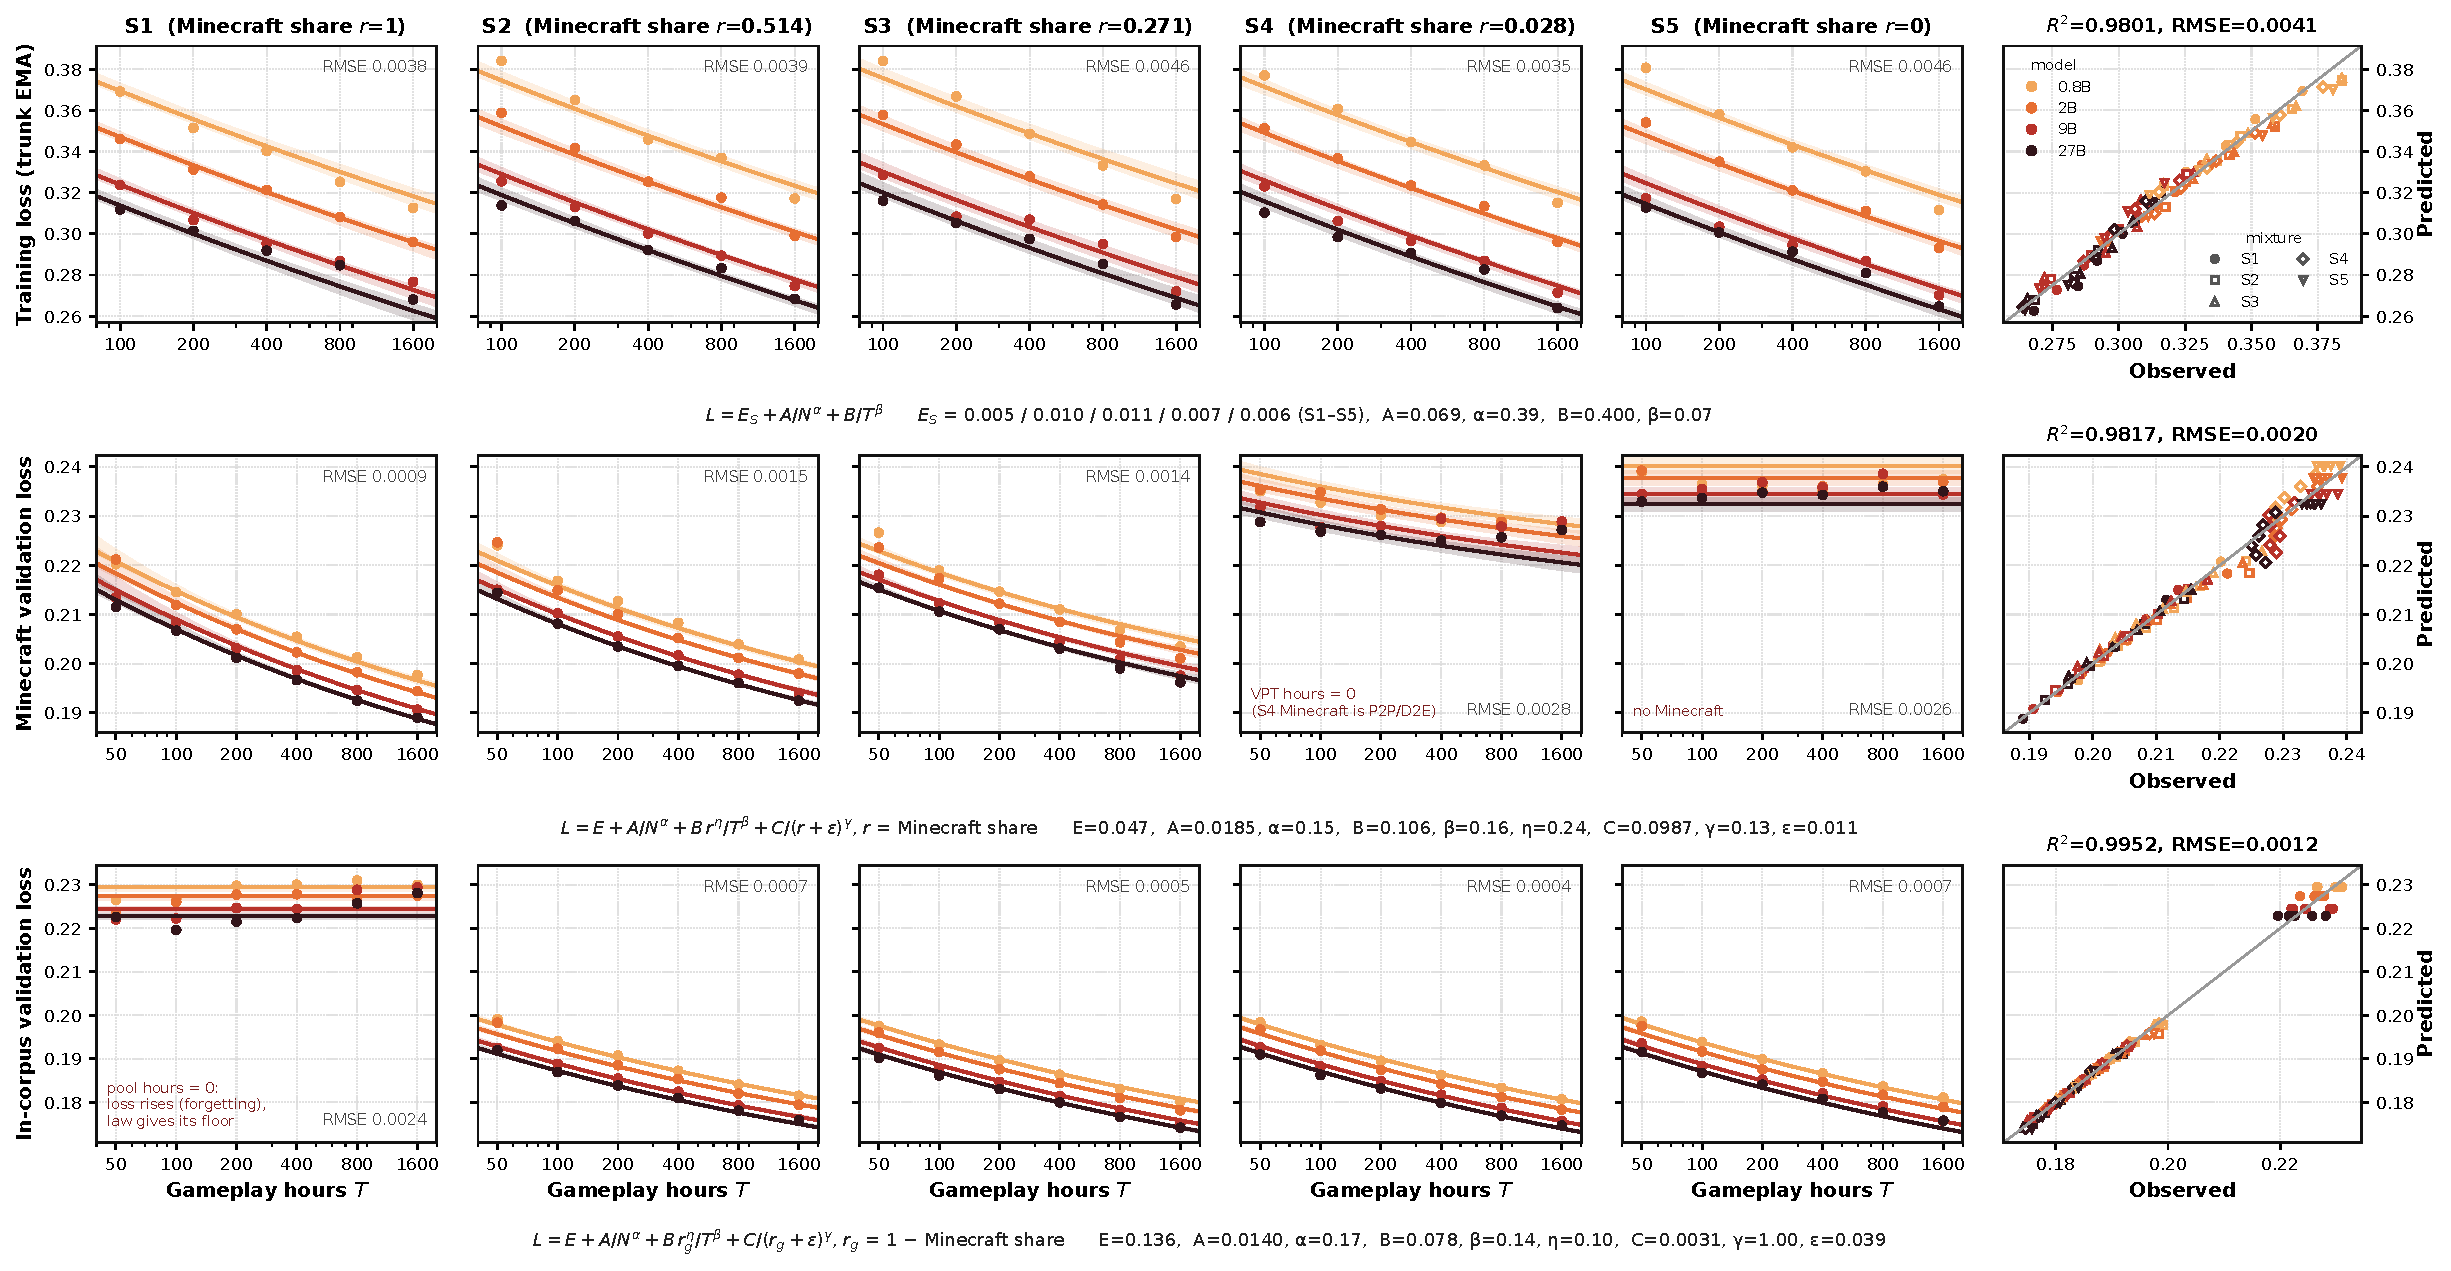
\includegraphics[width=0.97\linewidth]{figs/gamescaling_scaling_uncertainty.pdf}
    \caption{\textbf{Scaling-law fits with predictive uncertainty.} The panels show the training, Minecraft, and in-corpus loss laws across S1-S5, with measurements, predictions, and stratified-bootstrap bands. Prediction bands reflect variation across resampled experimental configurations within the observed grid, not seed-to-seed variance in model training.}
    \label{fig:gamescaling_uncertainty}
\end{figure*}

The composition-aware relation explains both differences among mixtures and their different slopes with respect to gameplay hours. An equally parameterized categorical-offset alternative cannot predict a held-out mixture and yields higher training-grid errors: Minecraft RMSE 0.0044 versus 0.0020 and in-corpus RMSE 0.0035 versus 0.0012. By contrast, distant unseen-game losses generally rise after the early interface phase, and their within-mixture scaling fit is weak. We therefore interpret the fitted relation as an empirical description of the measured in-corpus data regime rather than a universal law for unseen environments. Figure~\ref{fig:gamescaling_uncertainty} and Table~\ref{tab:scaling_holdout} demonstrate the fit's accuracy and limitations.

\subsection{Frontier-Model Progress and CPT Transfer}
\label{app:cpt_frontier_progress}

\begin{figure*}[t]
    \centering
    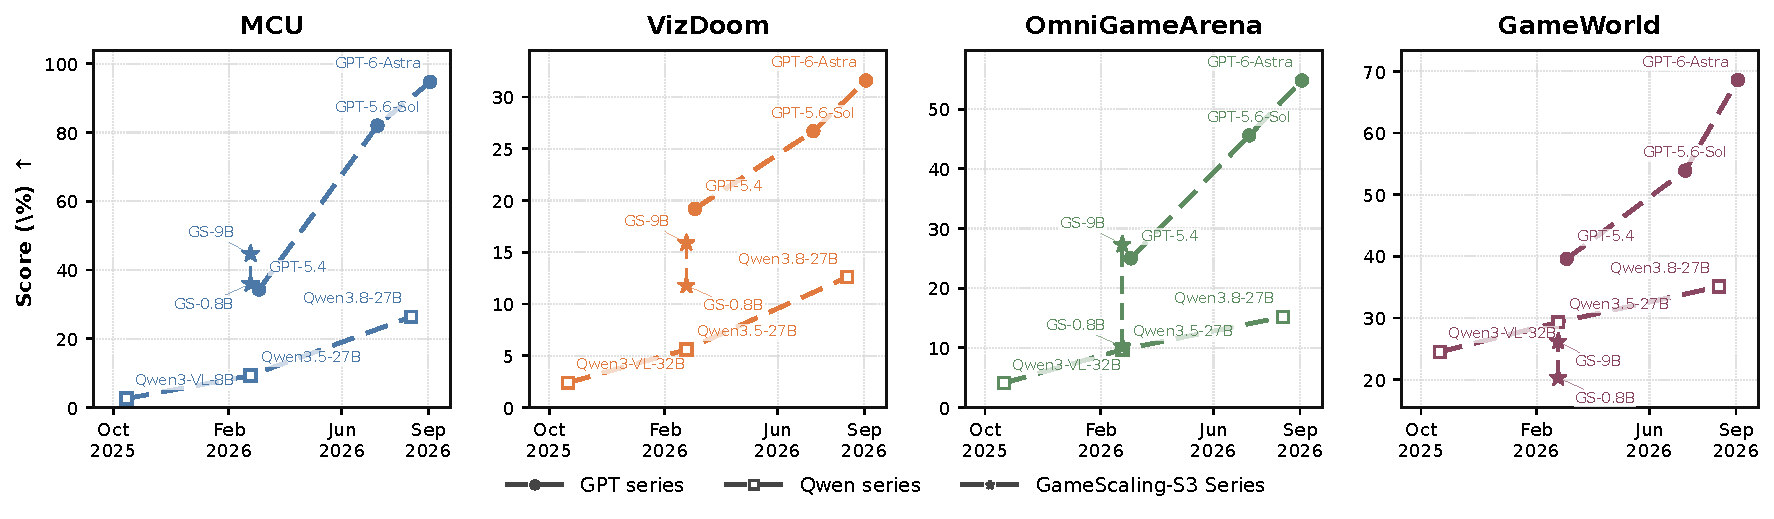
\includegraphics[width=0.92\linewidth]{figs/gamescaling_frontier_release_trends.pdf}
    \caption{\textbf{Frontier-model progress on four public game benchmarks.} Scores are plotted against model release date under time-paused evaluation. Circles indicate the GPT series, squares the Qwen series, and stars the GameScaling-S3 checkpoints at 1,600 gameplay hours (marked GS in the original plot). These results are from the controlled scaling study, not the HSR-augmented \ourmodel-CPT model. The comparison shows gains from gameplay adaptation alongside the contribution of general backbone capabilities, particularly on distant worlds.}
    \label{fig:cpt_frontier_progress}
\end{figure*}

Figure~\ref{fig:cpt_frontier_progress} places the GameScaling CPT checkpoints alongside successive general-purpose model releases on MCU, ViZDoom, OmniGameArena, and GameWorld. The controlled GameScaling results show that gameplay pretraining enables smaller backbones to achieve substantial gains on the source and related 3D environments. However, improvements across generations of general-purpose models are also pronounced, particularly on GameWorld, where distant-world transfer remains limited for the CPT checkpoints. The trends reflect progress from both game-specific adaptation and improvements to the underlying multimodal model. All points in this comparison use time-paused evaluation, so they characterize gameplay capability without conflating it with the real-time latency effects examined in the main experiments.

\subsection{Test-Time Interaction Budgets}
\label{app:cpt_test_time}
\begin{figure}[!htbp]
    \centering
    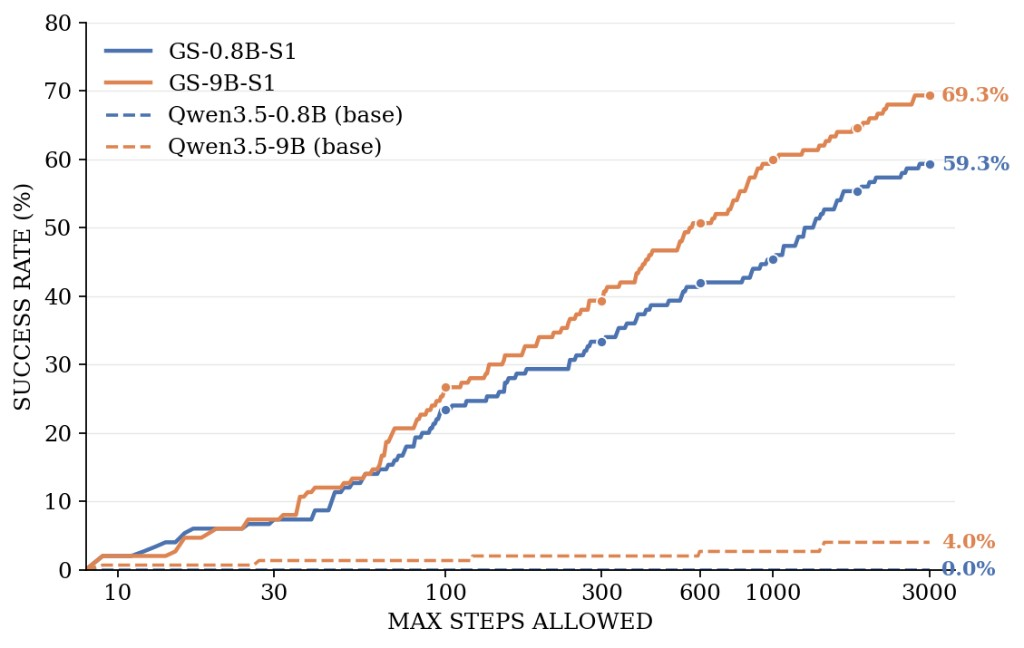
\includegraphics[width=0.74\linewidth]{figs/gamescaling_mcu_test_time.png}
    \caption{\textbf{Test-time scaling on MCU.} Cumulative task success versus available interaction steps (up to 3,000) for CPT checkpoints and unadapted Qwen3.5 backbones. The primary MCU protocol uses a 600-step cap. This supplementary sweep illustrates how additional interaction opportunities affect task completion.}
    \label{fig:gamescaling_test_time}
\end{figure}

As illustrated in Figure~\ref{fig:gamescaling_test_time}, increasing the test-time budget from 600 to 3,000 steps raises success for the CPT models in this comparison. The two reported checkpoints reach 59.3\% and 69.3\% at 3,000 steps, while the unadapted backbones remain near zero. A larger interaction budget helps policies that have already learned useful control, but cannot replace CPT. These curves are supplementary to the fixed-budget primary MCU scores.


\section{Streaming-vLLM Implementation Details}
\label{app:streaming_details}
\subsection{FSM-Guided Drafting and BF16 Verification}
\label{app:speculative_sampling}

\textbf{FSM grammar coverage.} The SM90 fast FSM recognizes the boundaries \texttt{<think>}, \texttt{</think>}, \texttt{<|action\_start|>}, and \texttt{<|action\_end|>}. It can draft the end of an empty reasoning span or the beginning of an action packet after a finished reasoning span. Within the XYZ mouse-coordinate fields, the FSM drafts formatting tokens following numerical values, not the coordinate values themselves. In the six subsequent key groups, it drafts predictable delimiters, blank-key templates, and the action terminator. Candidate tokens are proposed opportunistically when the current grammar state supports them.

\textbf{Target-model verification.} The drafts are checked by the target model before being committed. A candidate prefix is accepted only where each drafted token equals the token that target-model verification selects at the corresponding position under the active sampling rule (greedy argmax or temperature sampling); rejected suffixes and their speculative cache states are discarded. Throughout generation, the FSM simultaneously enforces grammar-level constrained decoding and speculative drafting: at every decoding and verification position, it restricts token selection to valid protocol transitions via state-dependent vocabulary bitmasks in the fused sampler---including for tokenizers whose action delimiters span multiple subword pieces---while proposing predictable structural continuations as drafts for parallel target-model verification, without replacing the policy's semantic action decisions over coordinate values or valid key combinations. 

\subsection{Incremental RoPE Cache Refresh}
\label{app:rope_refresh}

Figure~\ref{fig:rope_refresh_geometry} illustrates the incremental positional refresh used for retained KV states after context compaction.
A cached key originally associated with logical position $p$ may be reassigned to a new position $\widehat p$.
Rather than recomputing its key projection, Streaming-vLLM applies only the positional difference
\[
\Delta p
=
\widehat p-p.
\]

\begin{figure*}[t]
    \centering
    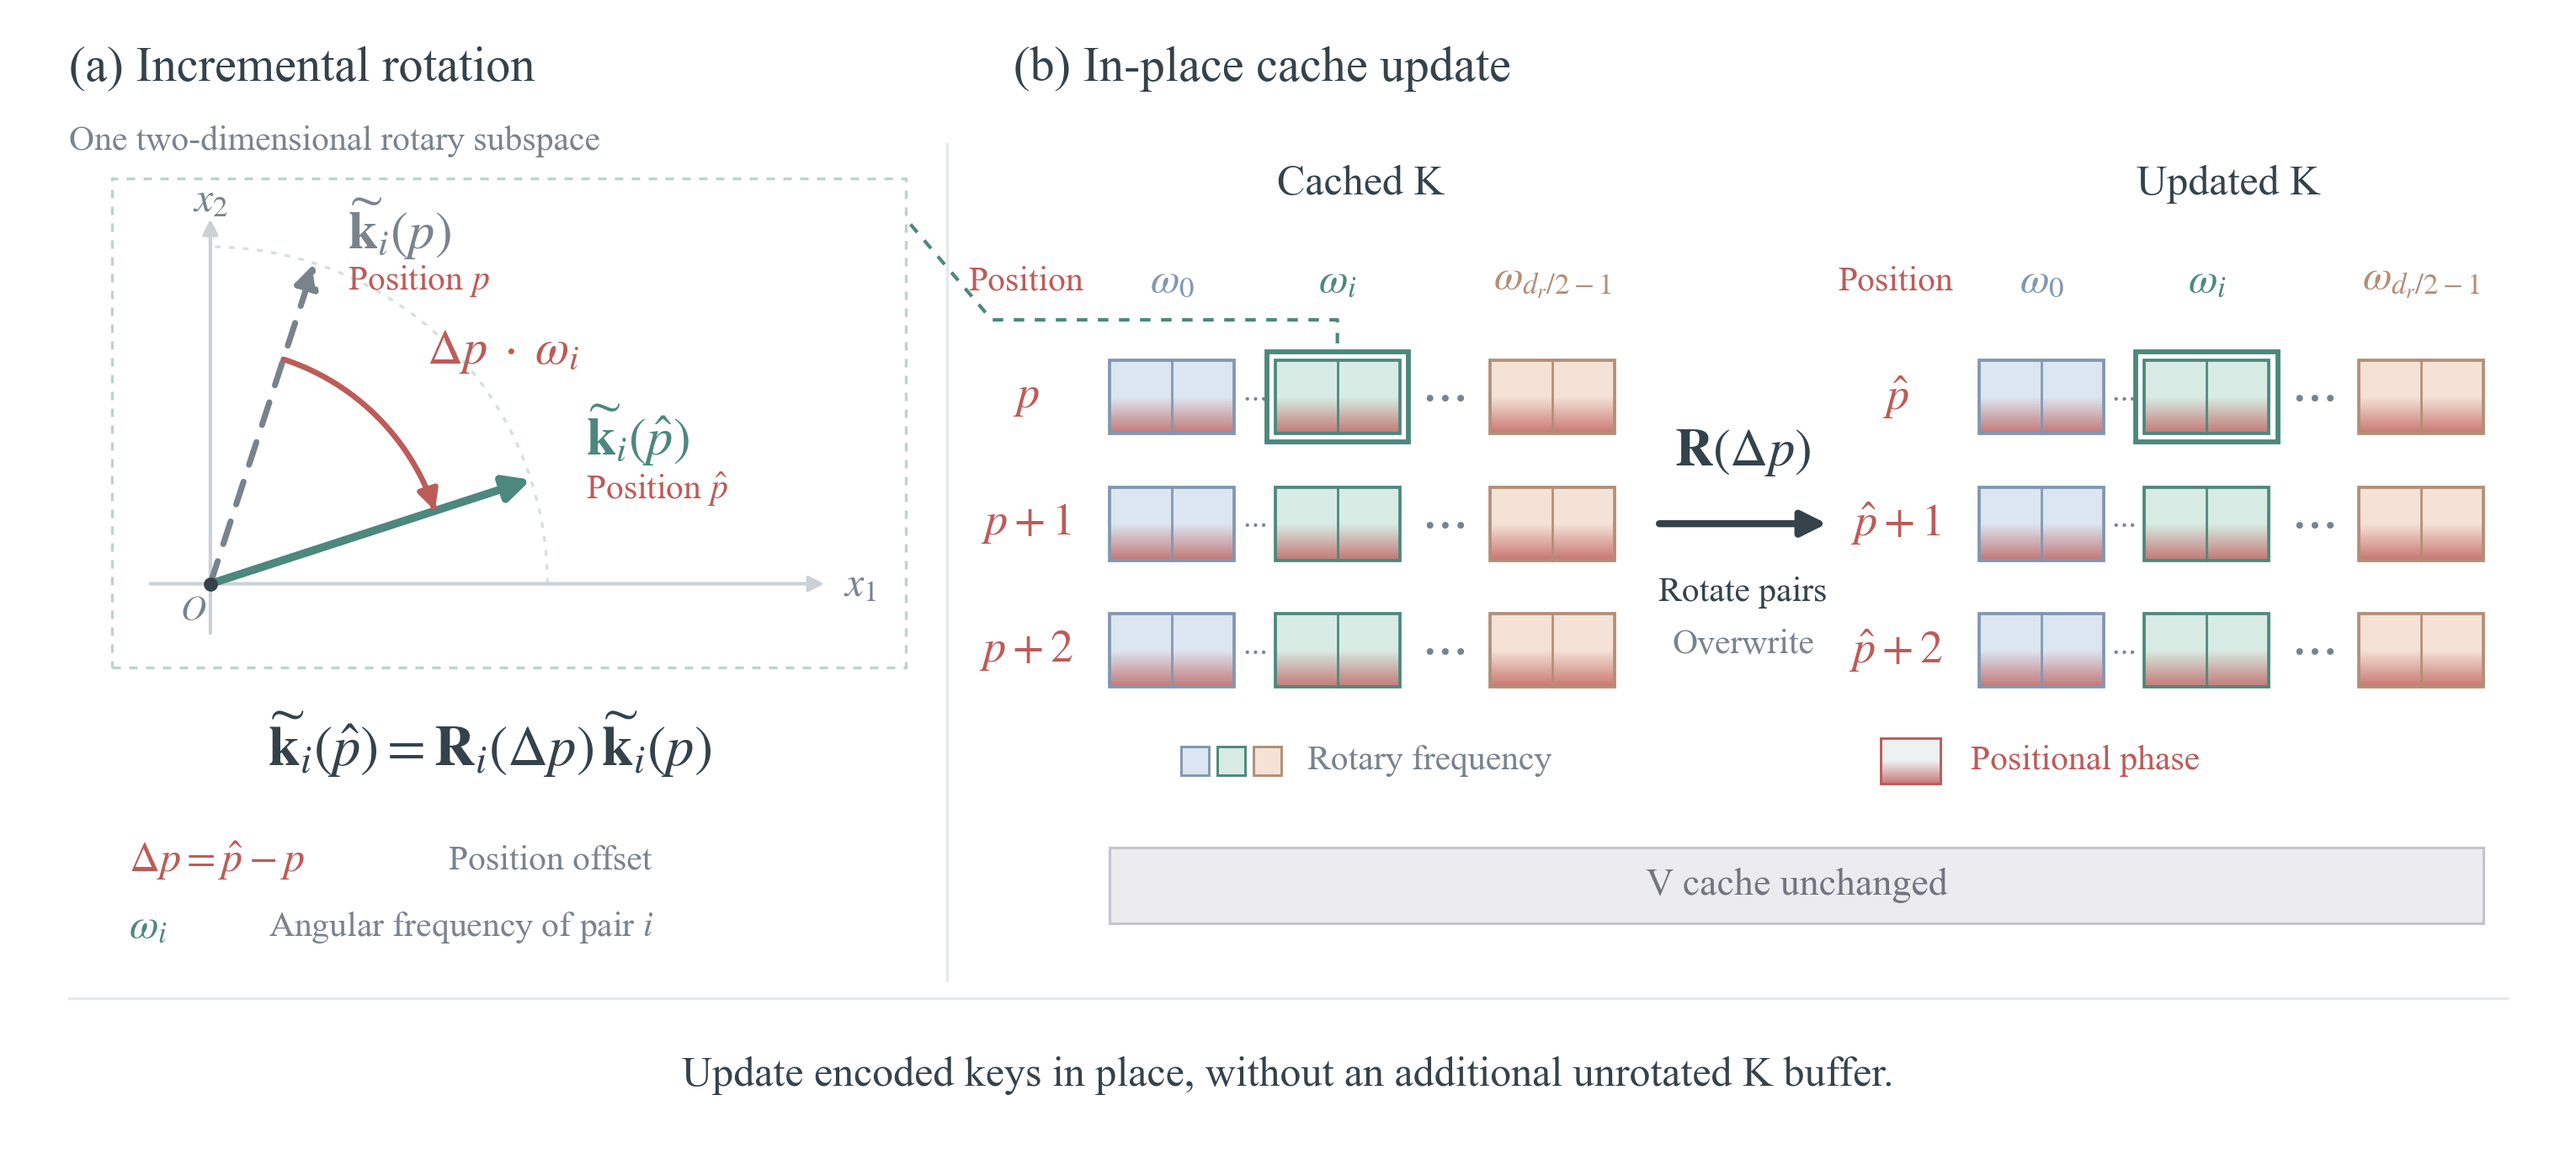
\includegraphics[width=0.85\linewidth]{figs/rope-position-refresh.png}
    \caption{
    \textbf{Incremental RoPE refresh for retained KV states.}
    A cached key moved from logical position $p$ to $\widehat p$ is updated by an additional rotation determined by $\Delta p=\widehat p-p$.
    The same positional offset is applied independently to each RoPE frequency pair and written back in place, while the value cache remains unchanged.
    The figure illustrates $\Delta p<0$, corresponding to a leftward shift after context compaction.
    }
    \label{fig:rope_refresh_geometry}
\end{figure*}

For a pair of cached key components $(u,v)$ associated with rotary frequency $\omega_i$, let
\[
\phi
=
\Delta p\,\omega_i.
\]
The incremental update is implemented as
\begin{equation}
\begin{aligned}
u'
&=
u\cos\phi-v\sin\phi,\\
v'
&=
u\sin\phi+v\cos\phi.
\end{aligned}
\label{eq:rope_pairwise_update}
\end{equation}

Both updated components are computed from the original pair before being written back to the cache.
The implementation follows the component-pair layout used by the underlying model and applies the corresponding update independently to all dimensions participating in RoPE.

Tokens whose logical positions remain unchanged have $\Delta p=0$ and therefore require no modification.
The update is performed in place on the retained key cache.
No unrotated key representation is stored, and the value cache is left unchanged.
For RoPE variants with multiple positional axes, the same correction is applied independently to the component groups associated with each axis.

This update corrects only the rotary positional phase.
As discussed in Sec.~\ref{sec:streaming_context}, retained KV states continue to follow the stateful streaming semantics of Streaming-vLLM rather than being reconstructed through full re-encoding after memory compaction.

\subsection{Hardware and Model-Architecture Coverage}
\label{app:streaming_architecture}

\textbf{Hardware mapping and evaluated backbones.} The Ampere measurements use NVIDIA A800 GPUs, while the Hopper measurements use NVIDIA H200 GPUs. Figure~\ref{fig:streaming_vllm_configuration_latency} compares Qwen3-VL-8B, a representative dense visual-language model, and Qwen3.5-35B-A3B, a representative mixture-of-experts model. Both are run with multiple tensor-parallel configurations and numerical precision settings. The Qwen3-VL and Qwen3.5 families are supported at additional dense and MoE sizes listed in Table~\ref{tab:training_recipe}, but this figure should not be read as an exhaustive per-checkpoint benchmark.

\textbf{Representative cross-hardware behavior.} Under TP4 and BF16, Qwen3-VL-8B has a mean request latency of 147.64 ms on datacenter Ampere and 75.66 ms on Hopper. Qwen3.5-35B-A3B has corresponding latencies of 205.77 ms and 110.08 ms. On Hopper, TP4 FP8 W8A8 further yields 74.69 ms and 92.19 ms, respectively. These figures come from the multi-turn latency-composition sweep and are not matched compute-cost comparisons across GPU generations. These results show that the same stateful serving design supports dense and MoE backbones on both architectures. The best parallelism and precision settings vary with the model and hardware.

\subsection{Latency Composition and Control-Rate Interpretation}
\label{app:streaming_latency}

The end-to-end request time comprises vision encoding, context processing, action generation, and runtime overhead. In the figure, Ampere denotes NVIDIA A800, and Hopper denotes NVIDIA H200. Figure~\ref{fig:streaming_vllm_configuration_latency} compares these components across model architectures, hardware generations, parallel settings, and numerical precision. The system ablation reports step rate (SR), the reciprocal of end-to-end request latency, and a theoretical control rate (CR) obtained by multiplying SR by the six low-level blocks in each action packet. CR is a latency-derived upper bound, not a direct measurement of the client execution cadence. The latter uses approximately 33~ms per block (30~Hz) when actions arrive in time.

\begin{figure*}[t]
    \centering
    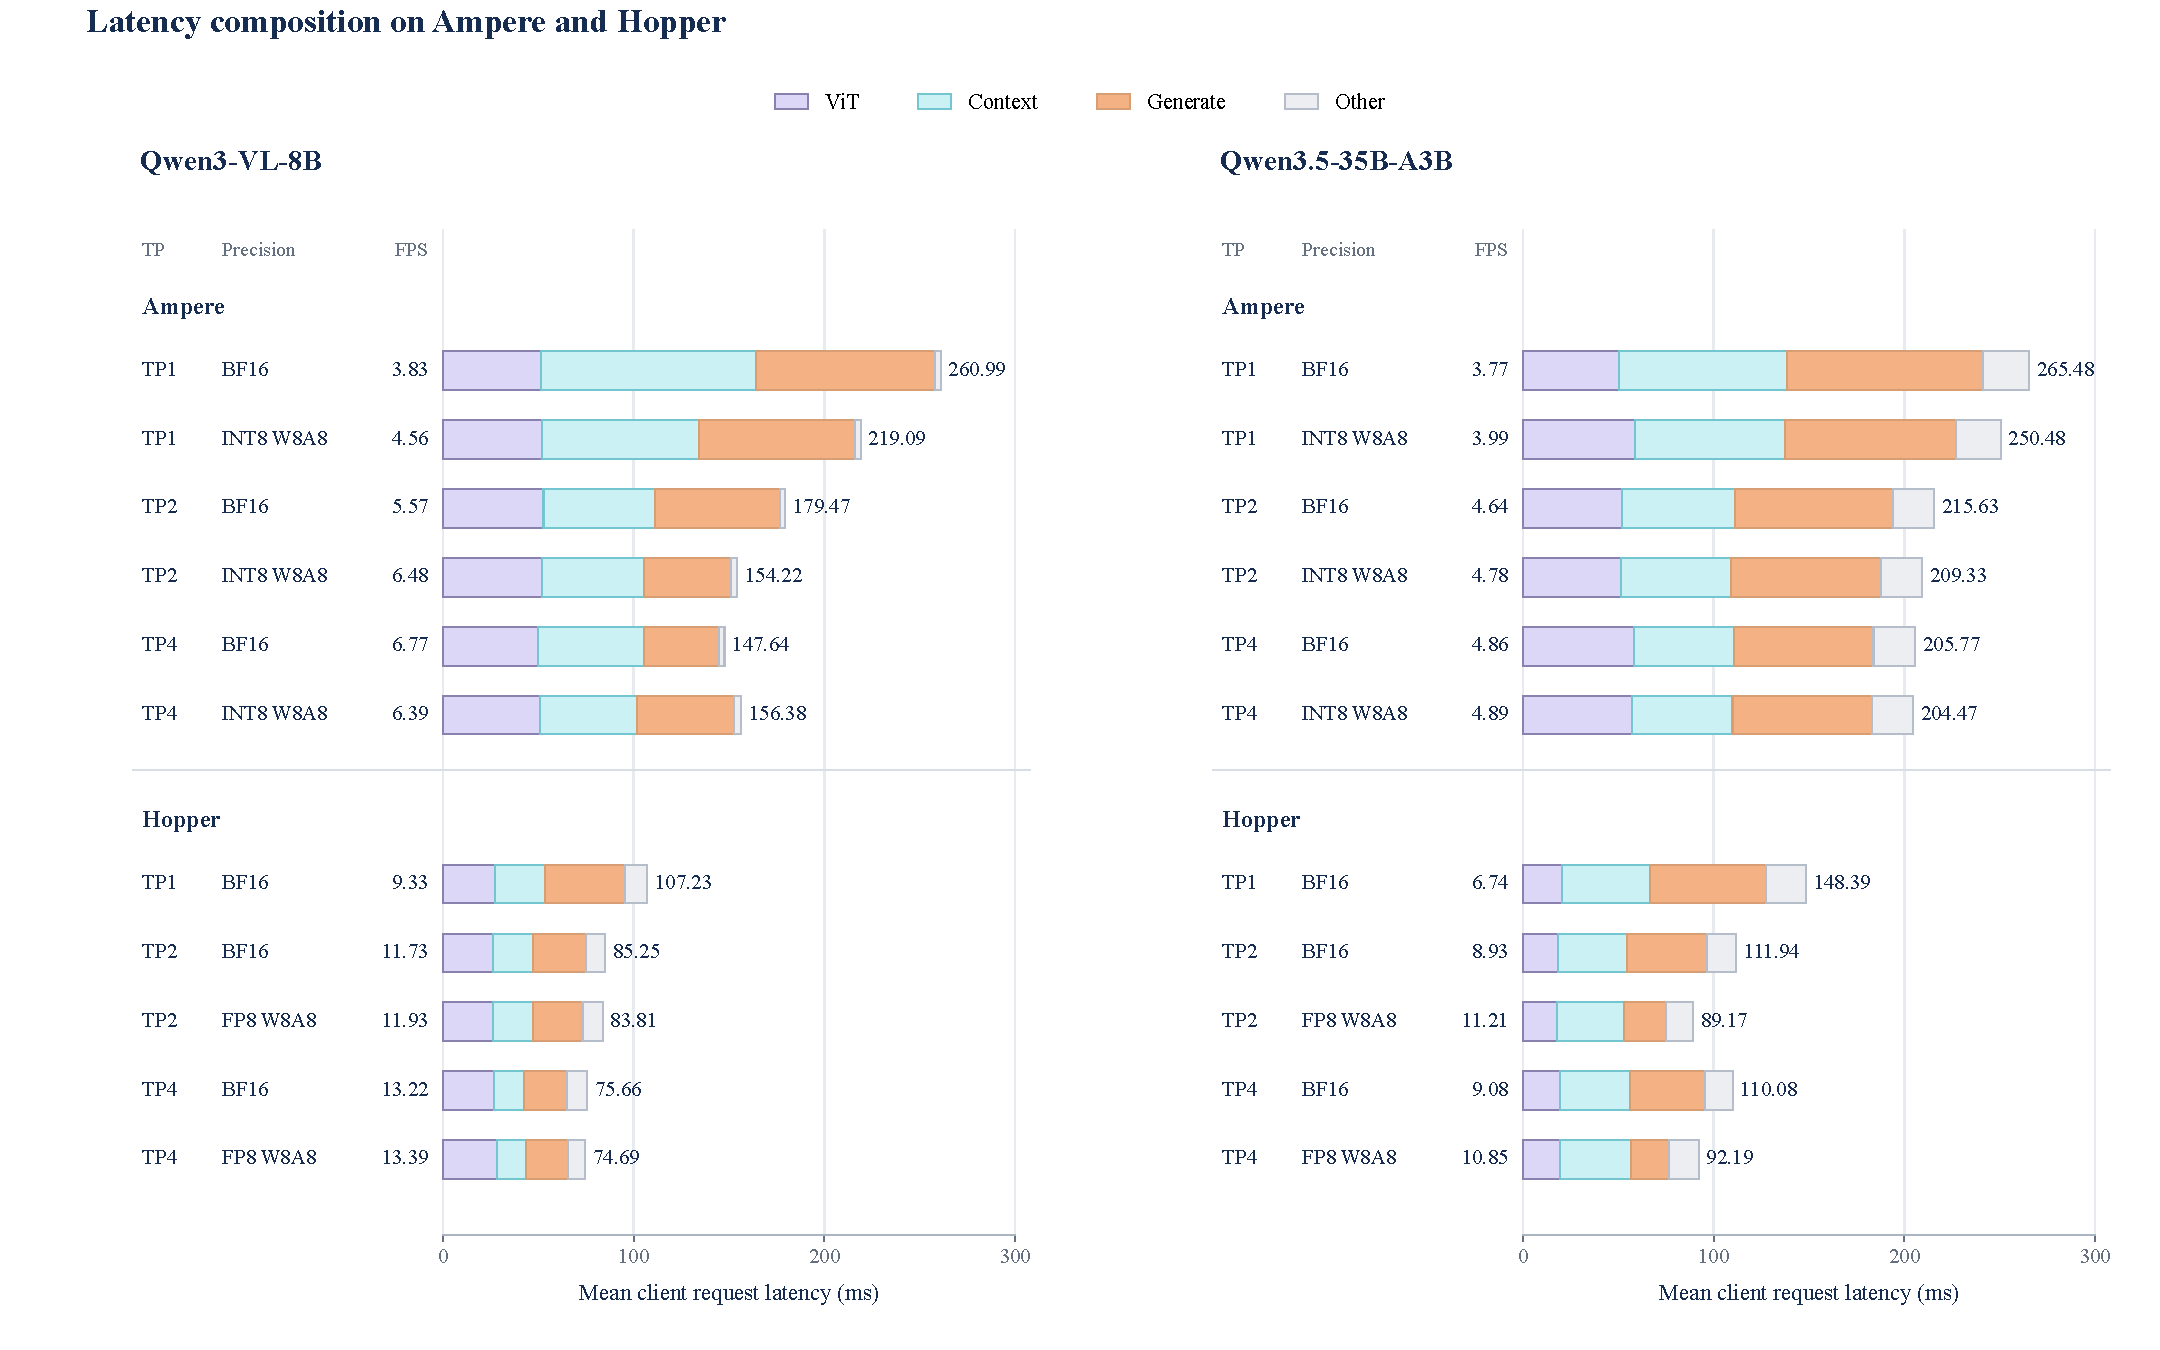
\includegraphics[width=\linewidth]{figs/latency-composition.pdf}
    \caption{\textbf{Cross-backbone request latency on NVIDIA A800 (Ampere) and H200 (Hopper).} The existing sweep compares Qwen3-VL-8B (Dense) and Qwen3.5-35B-A3B (MoE) across tensor-parallel degrees and BF16 or W8A8 execution. Stacked values separate vision processing, context (prefill), generation (decode), and remaining overhead, measured as mean request latency. These results characterize representative hardware and backbone coverage rather than all supported model sizes. The theoretical control rate in Table~\ref{tab:streaming_vllm_ablation} is derived from request time, not measured at the client.}
    \label{fig:streaming_vllm_configuration_latency}
\end{figure*}

\FloatBarrier

\section{Honkai: Star Rail Evaluation Protocol and Taxonomy}
\label{app:hsr_protocol}

\subsection{World Diversity and Interactive Complexity}
\label{app:hsr_world_diversity}

\textit{Honkai: Star Rail} provides a useful setting for studying generalist game agents because its complexity comes from combining familiar interactions across a large, varied world, rather than from a single difficult mechanic. Figure~\ref{fig:hsr_world_maps} brings together 171 floor maps from 85 areas across the game's major worlds. The maps range from compact rooms and branching corridors to large open layouts, interconnected structures, and multi-floor environments. Even when presented at a common coordinate scale, their differences are apparent. An agent cannot assume that a route learned in one area will work in another. It must adjust to new geometry, identify transitions between areas or floors, and preserve its destination as the scene changes.

\begin{figure*}[t]
    \centering
    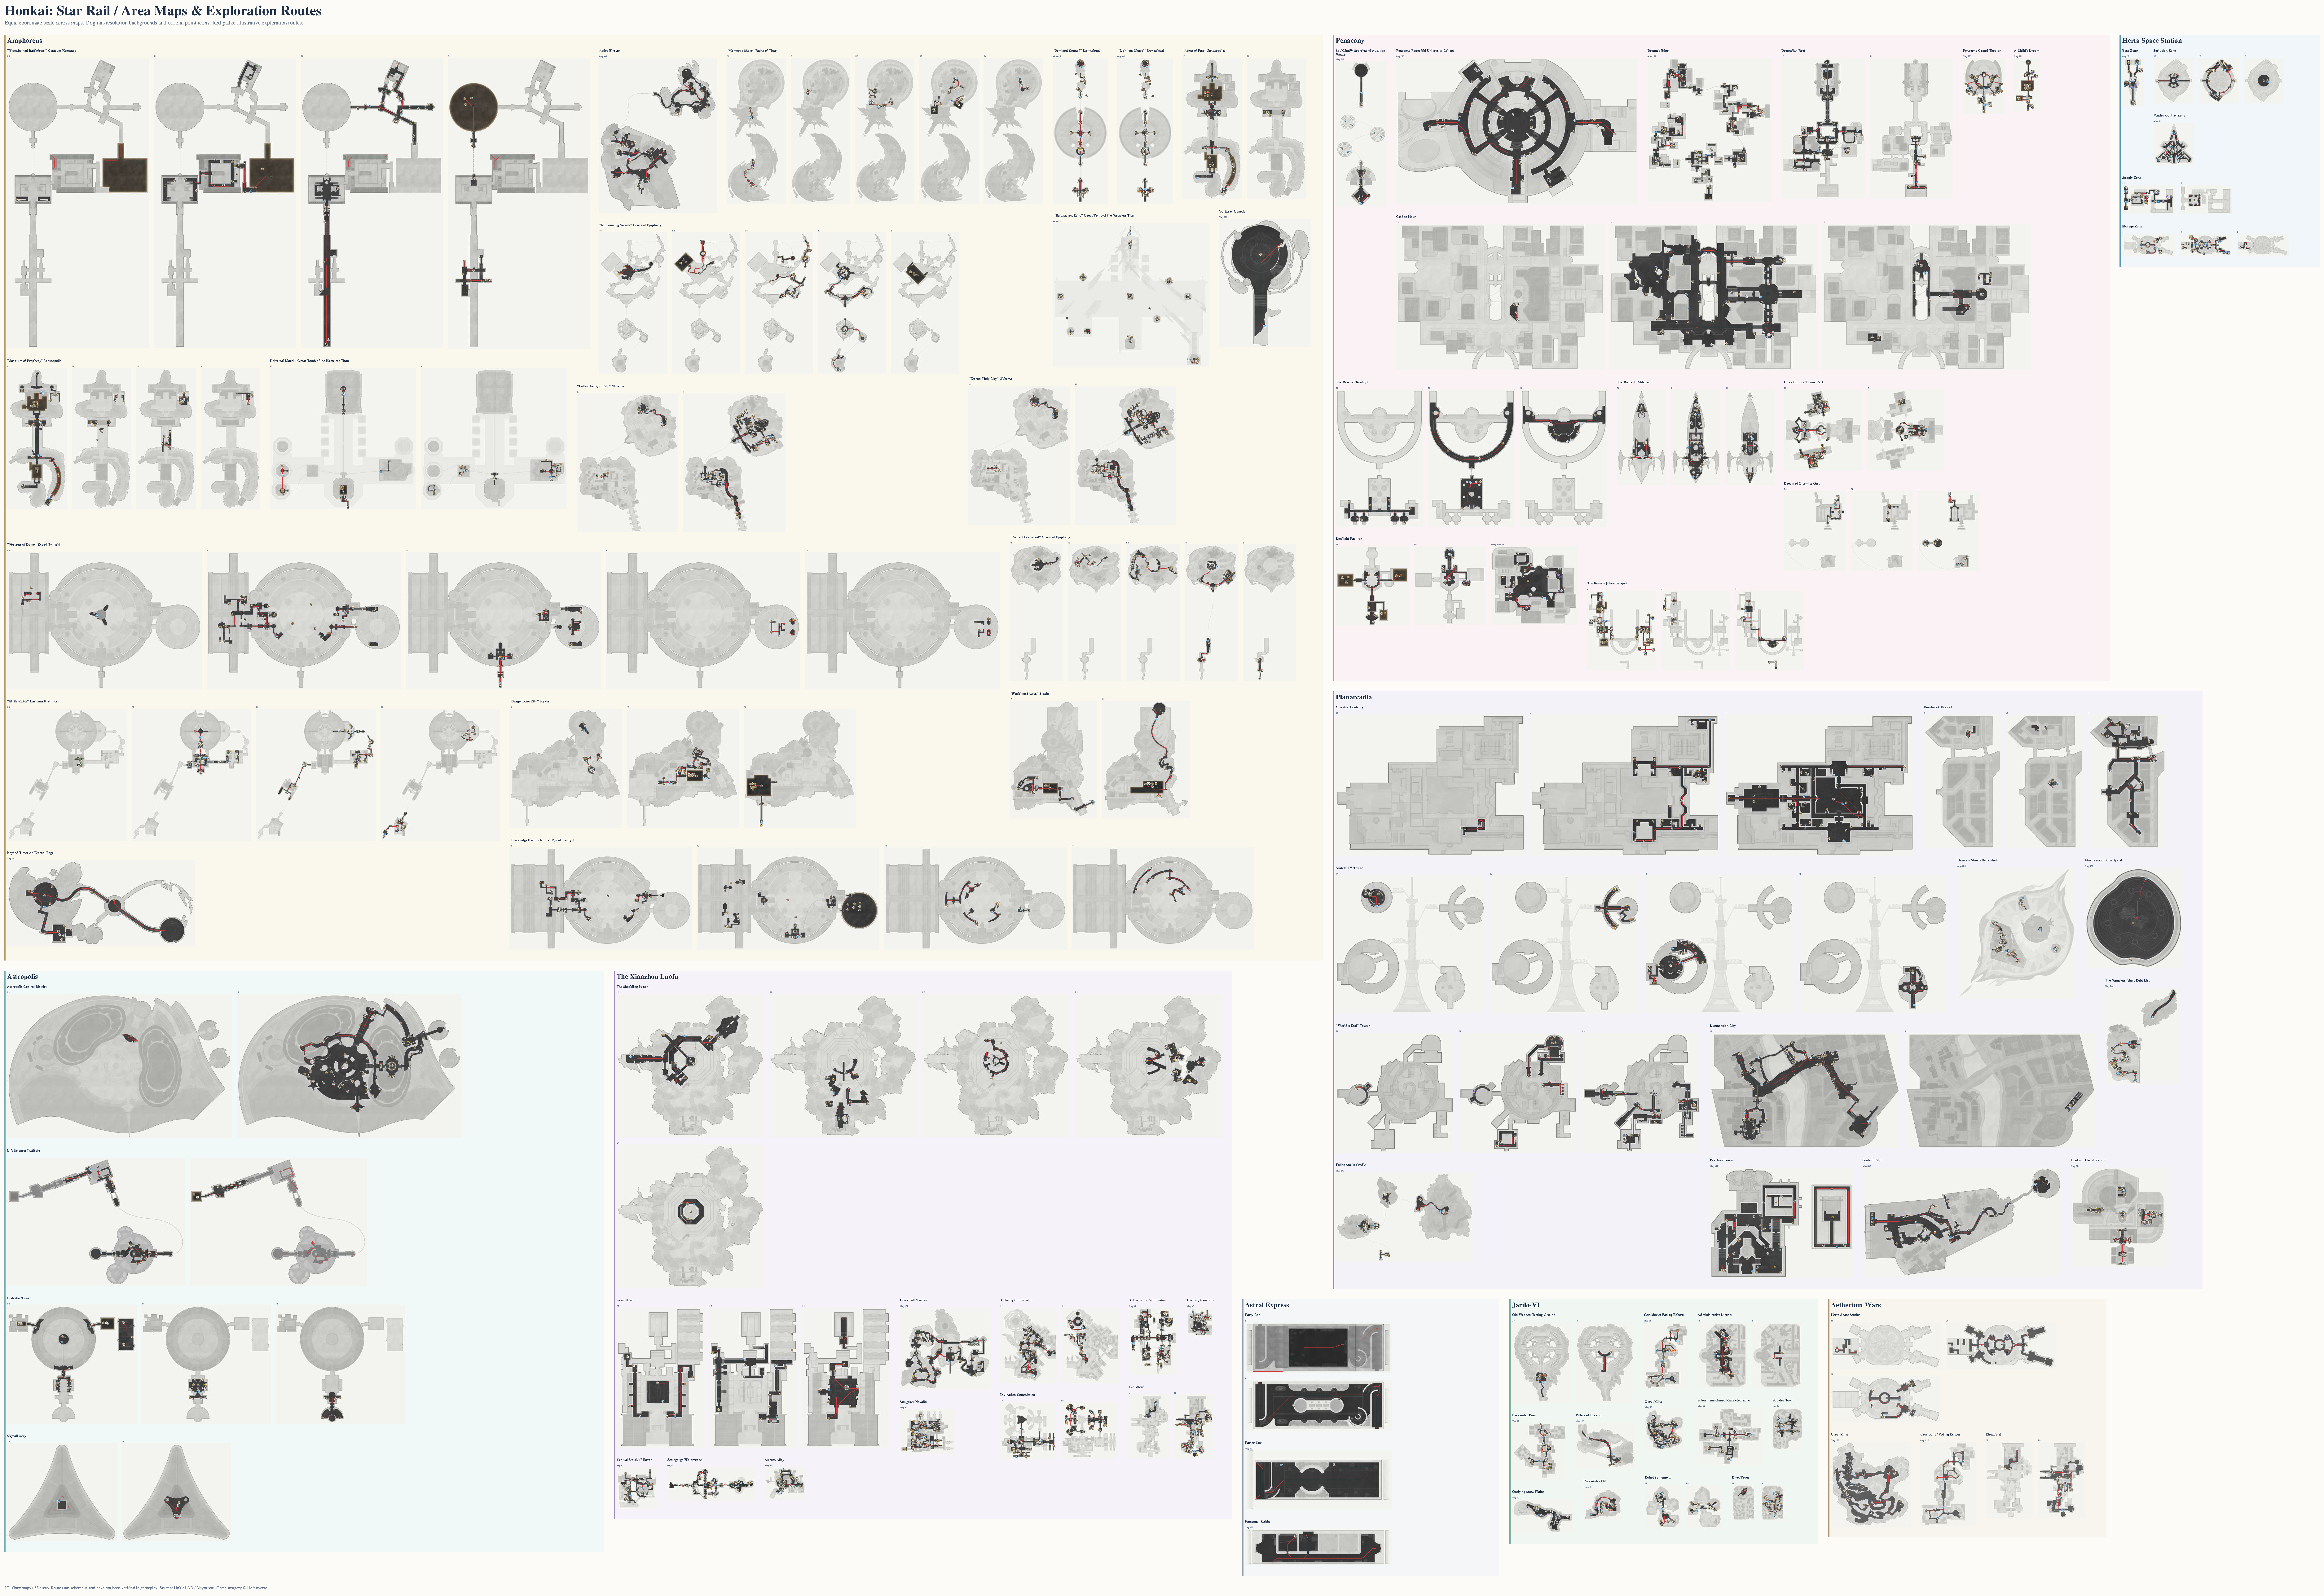
\includegraphics[width=0.92\textwidth]{figs/hsr_map.pdf}
    \caption{\textbf{Exploration diversity in \textit{Honkai: Star Rail}.}
    Map layouts vary in geometry, connectivity, and floor structure, and point icons indicate resources and other interactive locations. Red paths illustrate the possible exploration routes. }
    \label{fig:hsr_world_maps}
\end{figure*}
\FloatBarrier


The many point icons also reveal how exploration and task execution are interleaved. Individual areas contain resources and other points of interest alongside locations relevant to progression and interaction. A route can pass several optional objects before reaching the target, and the shortest visible path need not be a feasible sequence of game actions. The red paths in Figure~\ref{fig:hsr_world_maps} are \textbf{schematic exploration routes}, not gameplay-verified optimal solutions. They illustrate the need to plan through branching spaces, but do not establish that any particular route is the fastest or most reliable. The annotated maps are provided only to describe the environment and are \textbf{not given to the evaluated agents} as observations or privileged navigation input.

\textbf{Accessible gameplay does not imply easy autonomous control.} For a human player, quest objectives, map markers, and familiar interaction prompts make many individual steps understandable. A vision-language-action agent receives only the rendered screen and must turn this guidance into timed keyboard and mouse inputs. It must recognize where it is, distinguish relevant objects from nearby distractions, navigate while the camera and scene change, and determine when an interaction has actually completed. Longer tasks add another difficulty: navigation, dialogue, UI manipulation, combat, and local puzzles may appear within the same quest. Failure at one step can invalidate a later plan, and an agent must remember earlier progress even after those observations leave its active context. The challenge is therefore not simply to play any one minigame, but to coordinate heterogeneous skills over time.

This combination makes the game useful for both research and practical evaluation. Short interactive challenges probe whether a policy can adapt to different local rules, while side quests test whether those skills support sustained, instruction-conditioned progress. The same interface also reflects conditions faced by automated game testing: new content introduces routes, objects, objectives, and mechanics that cannot all be anticipated by hand-written scripts. A generalist agent able to execute these tasks through screen observations and device-level actions could support exploration, quest verification, and regression testing without modifications to the game engine. These are \textbf{potential applications}, not deployment benefits measured by the map itself. Our experiments cover a defined subset of this broader environment. Although \ourmodel-CPT is trained on other \textit{Honkai: Star Rail} gameplay, neither of the two evaluated side quests nor any of the 40 scored minigame tasks is included in training. This split tests generalization to held-out tasks within a familiar game world, not zero-shot transfer to a game unseen during training.


\subsection{Combat Mechanics and Strategic Decision-Making}
\label{app:hsr_combat}

\begin{figure}[H]
    \centering
    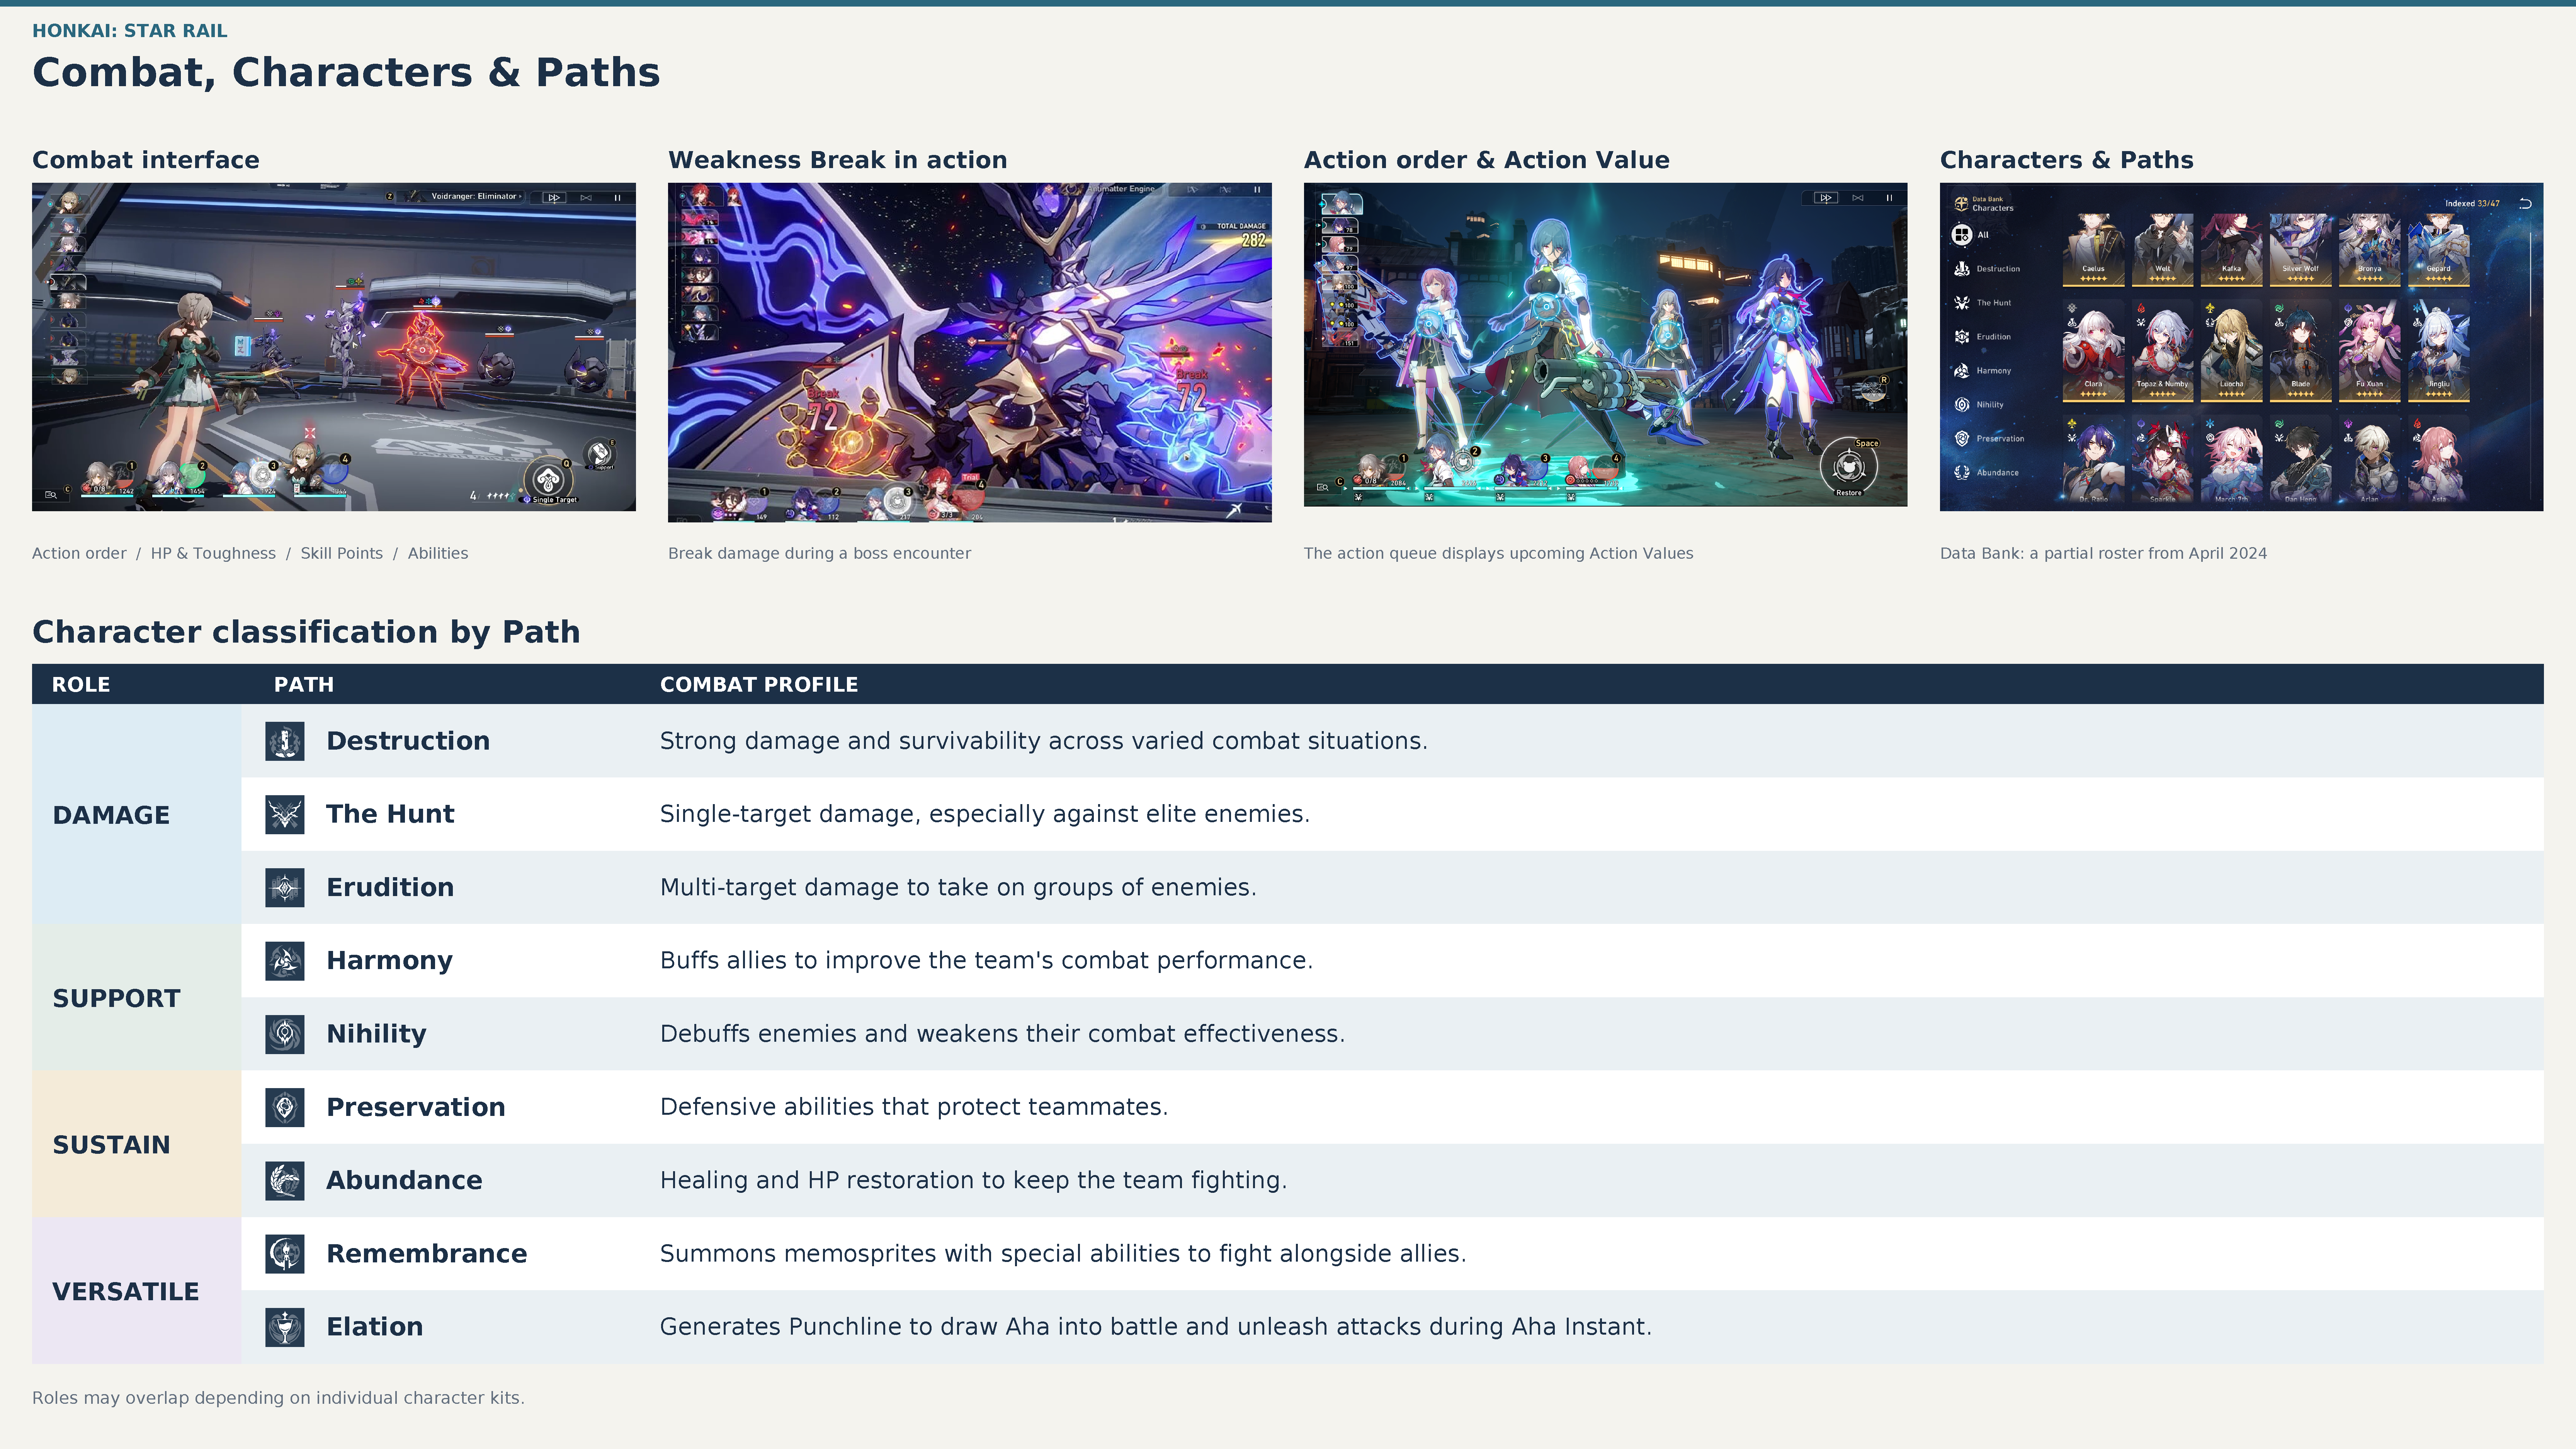
\includegraphics[width=0.70\linewidth]{figs/hsr_combat.pdf}
    \caption{\textbf{Combat mechanics and character roles in \textit{Honkai: Star Rail}.} The examples illustrate (1) the combat interface, including action order, HP and Toughness, team status, skill points, and available abilities, (2) a Weakness Break during a boss encounter, (3) the Action Value display, and (4) a character Data Bank snapshot. The lower panel summarizes the nine Paths by representative combat roles, including damage, support, sustain, and more specialized mechanics. Path groupings summarize representative combat roles, and the figure provides game-mechanics context rather than a measured policy rollout.}
    \label{fig:hsr_combat_mechanics}
\end{figure}

Exploration is only one part of \textit{Honkai: Star Rail}. Combat adds a different decision-making problem within the same game interface. The game uses turn-based encounters, but choosing an action still depends on information that changes throughout the fight. As shown in Figure~\ref{fig:hsr_combat_mechanics}, the combat screen combines the action-order queue with character HP, enemy Toughness, team status, skill points, and available abilities. The action-order display and Action Value indicate when combatants will act, while the Toughness system creates opportunities for Weakness Break. The agent must use these cues together, rather than treating each turn as an isolated image-to-action decision.



Combat decisions involve coupled constraints over multiple turns. Attacking a vulnerable target may advance a Weakness Break, but the agent must also consider the available skill points, the health and status of its team, and which combatant acts next. Character roles introduce further variation. The Paths shown in Figure~\ref{fig:hsr_combat_mechanics} span single-target and multi-target damage, buffs and debuffs, protection and healing, summons, and other specialized combat effects. A useful action can therefore depend on the team composition and on how one character's choice changes the options available to others. Although human players can read these cues from a familiar interface, an autonomous policy must recognize them visually, choose a suitable action, and issue the corresponding executable inputs.

This makes combat complementary to the game's navigation, dialogue, and puzzle mechanics. Navigation requires spatial grounding and route execution, whereas combat requires state-dependent target selection and coordination of limited resources across turns. Both demand that the agent preserve its objective while the available actions and relevant observations change. The held-out side-quest benchmark includes combat milestones alongside other interaction types. The atlas in Figure~\ref{fig:hsr_combat_mechanics} provides context for those milestones and the broader game setting, rather than constituting a separate combat benchmark or evidence of a model's combat performance. Together with the exploration maps, it illustrates why generalist gameplay requires more than a collection of fixed action scripts: the same visual-control policy must adapt to different rules, time scales, and notions of progress within one evolving game world.


\subsection{Long-Horizon Milestones}

The long-horizon benchmark consists of two fixed quest specifications. \emph{Opportunity Makes the Thief (Part I)} contains 30 evaluation milestones grouped into 22 parent steps, with 14 navigation, 14 dialogue, one combat, and one UI milestone. \emph{Bestial Ferocity} contains 55 milestones grouped into 40 parent steps, with 32 navigation, 16 dialogue, two combat, two UI, and three puzzle milestones. Configured time budgets are attached to each required milestone. They are limits for evaluation, not observations of how long an agent took to complete a step. The ordering and terminal conditions are listed in Tables~\ref{tab:museum_milestones} and~\ref{tab:bestial_milestones}.

For each model, the milestone-type rate is the number of verified passes divided by the total milestones of that type in the respective quest. Quest accuracy uses all required milestones as its denominator rather than averaging type-level rates. If a run resumes through a scripted transition, a verified milestone pass does not establish uninterrupted autonomous progress. Missing evaluations are not counted as failures. The published report should state the exact number of valid attempts per model and task when final results are available.

\begin{table}[t]
\centering
\caption{\footnotesize \textbf{Opportunity Makes the Thief (Part I).} The 30 required milestones span 22 parent steps and cover navigation, dialogue, combat, and exhibit recovery. Read down the left block, then the right block.}
\label{tab:museum_milestones}
\vspace{5pt}
\footnotesize
\setlength{\tabcolsep}{2pt}
\renewcommand{\arraystretch}{1.06}
\begin{minipage}[t]{0.485\linewidth}
\vspace{0pt}
\centering
\textbf{First 15 milestones}\par
\vspace{4pt}
\begin{tabular*}{\linewidth}{@{}p{0.12\linewidth}@{\hspace{5pt}}p{0.66\linewidth}@{\extracolsep{\fill}}cr@{}}
\noalign{\hrule height 0.7pt}
\rule{0pt}{12pt}\textbf{ID} & \textbf{Milestone} & \textbf{Type} & \textbf{s} \\[2pt]
\hline
\noalign{\vskip 3pt}
1 & \raggedright Follow the quest marker to locate Pela. & N & 60 \\[0.5pt]
2 & \raggedright Talk to Pela and transition into the museum. & D & 60 \\[0.5pt]
3 & \raggedright Continue the conversation with Pela inside the museum. & D & 60 \\[0.5pt]
4 & \raggedright Follow Pela to the exhibit. & N & 120 \\[0.5pt]
5 & \raggedright Complete the conversation and transition to the Underworld. & D & 60 \\[0.5pt]
6 & \raggedright Finish the current conversation. & D & 60 \\[0.5pt]
7 & \raggedright Follow the quest marker to locate Swetta. & N & 60 \\[0.5pt]
8 & \raggedright Complete the conversation with Swetta. & D & 60 \\[0.5pt]
9.2a & \raggedright Locate and inspect the poster. & N & 180 \\[0.5pt]
9.2b & \raggedright Advance the dialogue associated with the poster. & D & 30 \\[0.5pt]
9.3a & \raggedright Approach the robot guards. & N & 180 \\[0.5pt]
9.3b & \raggedright Advance the dialogue until combat begins. & D & 30 \\[0.5pt]
9.3c & \raggedright Defeat the robot guards. & C & 120 \\[0.5pt]
9.3d & \raggedright Locate the crate containing a clue. & N & 30 \\[0.5pt]
9.3e & \raggedright Complete the dialogue associated with the crate. & D & 30 \\[0.5pt]
\noalign{\vskip 2pt}
\noalign{\hrule height 0.7pt}
\end{tabular*}
\end{minipage}
\hfill
\begin{minipage}[t]{0.485\linewidth}
\vspace{0pt}
\centering
\textbf{Final 15 milestones}\par
\vspace{4pt}
\begin{tabular*}{\linewidth}{@{}p{0.12\linewidth}@{\hspace{5pt}}p{0.66\linewidth}@{\extracolsep{\fill}}cr@{}}
\noalign{\hrule height 0.7pt}
\rule{0pt}{12pt}\textbf{ID} & \textbf{Milestone} & \textbf{Type} & \textbf{s} \\[2pt]
\hline
\noalign{\vskip 3pt}
9.1a & \raggedright Find the little girl and listen to the conversation. & N & 60 \\[0.5pt]
9.1b & \raggedright Complete the associated dialogue. & D & 30 \\[0.5pt]
10 & \raggedright Follow the quest marker to locate Pela. & N & 120 \\[0.5pt]
11 & \raggedright Advance the dialogue until the phone message interface opens. & D & 30 \\[0.5pt]
12 & \raggedright Complete the conversation in the phone message interface. & U & 30 \\[0.5pt]
13 & \raggedright Finish the subsequent conversation. & D & 30 \\[0.5pt]
14 & \raggedright Open the map and teleport to the next quest location. & N & 60 \\[0.5pt]
15 & \raggedright Locate and enter the cheap room. & N & 30 \\[0.5pt]
16 & \raggedright Interact with the clue inside the room. & N & 30 \\[0.5pt]
17 & \raggedright Complete the associated dialogue. & D & 30 \\[0.5pt]
18 & \raggedright Teleport back to the Administrative District. & N & 60 \\[0.5pt]
19 & \raggedright Locate the museum ticket inspector. & N & 60 \\[0.5pt]
20 & \raggedright Complete the conversation and enter the museum. & D & 30 \\[0.5pt]
21 & \raggedright Reach the target location and return the Meteor Stone fragment. & N & 30 \\[0.5pt]
22 & \raggedright Complete the final dialogue and finish the mission. & D & 30 \\[0.5pt]
\noalign{\vskip 2pt}
\noalign{\hrule height 0.7pt}
\end{tabular*}
\end{minipage}
\par\vspace{7pt}
\begin{minipage}{\linewidth}
\footnotesize
\textbf{Total: 30 milestones}\hfill\textbf{Time budget: 1,800 s}\par
\vspace{4pt}
\raggedright
\textbf{Types.} N: navigation (14), D: dialogue (14), C: combat (1), U: UI interaction (1).\par
\vspace{2pt}
\textbf{Notes.} IDs, order, and types follow the benchmark specification. Times are configured per-milestone budgets in seconds, not measured completion times.
\end{minipage}
\end{table}

\begin{table}[t]
\centering
\caption{\footnotesize \textbf{Bestial Ferocity.} The 55 required milestones span 40 parent steps and include three automaton-repair puzzles. Read down the left block, then the right block.}
\label{tab:bestial_milestones}
\vspace{5pt}
\footnotesize
\setlength{\tabcolsep}{2pt}
\renewcommand{\arraystretch}{1.06}
\begin{minipage}[t]{0.485\linewidth}
\vspace{0pt}
\centering
\textbf{First 28 milestones}\par
\vspace{4pt}
\begin{tabular*}{\linewidth}{@{}p{0.12\linewidth}@{\hspace{5pt}}p{0.66\linewidth}@{\extracolsep{\fill}}cr@{}}
\noalign{\hrule height 0.7pt}
\rule{0pt}{12pt}\textbf{ID} & \textbf{Milestone} & \textbf{Type} & \textbf{s} \\[2pt]
\hline
\noalign{\vskip 3pt}
1 & \raggedright Locate the unidentified NPC in Central Starskiff Haven. & N & 90 \\[0.5pt]
2 & \raggedright Complete the initial NPC dialogue. & D & 90 \\[0.5pt]
3 & \raggedright Teleport to Exalting Sanctum. & N & 90 \\[0.5pt]
4 & \raggedright Enter the Realm-Keeping Commission Chancery. & N & 90 \\[0.5pt]
5 & \raggedright Locate Jingyan. & N & 90 \\[0.5pt]
6 & \raggedright Complete the dialogue with Jingyan. & D & 120 \\[0.5pt]
7 & \raggedright Teleport to Scalegorge Waterscape. & N & 90 \\[0.5pt]
8 & \raggedright Reach the marked quest destination. & N & 90 \\[0.5pt]
9 & \raggedright Activate the Diting tracking trail. & N & 10 \\[0.5pt]
10 & \raggedright Follow the blue trail to the enemies. & N & 180 \\[0.5pt]
11 & \raggedright Advance the dialogue and defeat the enemies. & C & 180 \\[0.5pt]
12 & \raggedright Complete the post-encounter dialogue. & D & 90 \\[0.5pt]
13 & \raggedright Teleport to the Alchemy Commission. & N & 90 \\[0.5pt]
14 & \raggedright Reach Zhongshan and complete the dialogue. & N & 90 \\[0.5pt]
15 & \raggedright Talk to Zhongshan again. & D & 120 \\[0.5pt]
16 & \raggedright Reach the highlighted quest location. & N & 120 \\[0.5pt]
17 & \raggedright Open the phone and finish the messages. & U & 90 \\[0.5pt]
18 & \raggedright Find Zhongshan and continue the dialogue. & N & 90 \\[0.5pt]
19.1a & \raggedright Approach Heathmann to hear his request. & N & 90 \\[0.5pt]
19.1b & \raggedright Complete the dialogue with Heathmann. & D & 90 \\[0.5pt]
19.2a & \raggedright Approach Tonya to hear her request. & N & 90 \\[0.5pt]
19.2b & \raggedright Complete the dialogue with Tonya. & D & 90 \\[0.5pt]
19.3a & \raggedright Approach Benna to hear her request. & N & 90 \\[0.5pt]
19.3b & \raggedright Complete the dialogue with Benna. & D & 90 \\[0.5pt]
20 & \raggedright Finish the remaining Zhongshan dialogue. & D & 120 \\[0.5pt]
21 & \raggedright Teleport to the Silvermane Guard Restricted Zone. & N & 90 \\[0.5pt]
22 & \raggedright Locate Serval. & N & 120 \\[0.5pt]
23 & \raggedright Complete the dialogue with Serval. & D & 120 \\[0.5pt]
\noalign{\vskip 2pt}
\noalign{\hrule height 0.7pt}
\end{tabular*}
\end{minipage}
\hfill
\begin{minipage}[t]{0.485\linewidth}
\vspace{0pt}
\centering
\textbf{Final 27 milestones}\par
\vspace{4pt}
\begin{tabular*}{\linewidth}{@{}p{0.12\linewidth}@{\hspace{5pt}}p{0.66\linewidth}@{\extracolsep{\fill}}cr@{}}
\noalign{\hrule height 0.7pt}
\rule{0pt}{12pt}\textbf{ID} & \textbf{Milestone} & \textbf{Type} & \textbf{s} \\[2pt]
\hline
\noalign{\vskip 3pt}
24 & \raggedright Repair the Automaton Grizzly. & P & 180 \\[0.5pt]
25 & \raggedright Repair the Automaton Spider. & P & 180 \\[0.5pt]
26 & \raggedright Repair the Automaton Direwolf. & P & 180 \\[0.5pt]
27 & \raggedright Return to Scalegorge Waterscape. & N & 90 \\[0.5pt]
28 & \raggedright Follow the quest marker to Zhongshan. & N & 120 \\[0.5pt]
29 & \raggedright Complete the dialogue with Zhongshan. & D & 120 \\[0.5pt]
30.1a & \raggedright Approach Benna to discuss the mechanical creatures. & N & 90 \\[0.5pt]
30.1b & \raggedright Complete the dialogue with Benna. & D & 90 \\[0.5pt]
30.2a & \raggedright Approach Heathmann to discuss the mechanical creatures. & N & 90 \\[0.5pt]
30.2b & \raggedright Complete the dialogue with Heathmann. & D & 90 \\[0.5pt]
30.3a & \raggedright Approach Tonya to discuss the mechanical creatures. & N & 90 \\[0.5pt]
30.3b & \raggedright Complete the battle and its preceding and following dialogues. & C & 180 \\[0.5pt]
31 & \raggedright Reach Zhongshan and initiate dialogue. & N & 120 \\[0.5pt]
32 & \raggedright Complete the group dialogue. & N & 180 \\[0.5pt]
33 & \raggedright Complete the text-message conversation. & U & 180 \\[0.5pt]
34 & \raggedright Reach Nannan and initiate dialogue. & N & 120 \\[0.5pt]
35 & \raggedright Complete the Nannan and Zhongshan dialogue. & N & 120 \\[0.5pt]
36.1a & \raggedright Visit Benna to check on her situation. & N & 90 \\[0.5pt]
36.1b & \raggedright Complete the dialogue with Benna. & D & 90 \\[0.5pt]
36.2a & \raggedright Visit Tonya to check on her situation. & N & 90 \\[0.5pt]
36.2b & \raggedright Complete the dialogue with Tonya. & D & 90 \\[0.5pt]
36.3a & \raggedright Visit Heathmann to check on his situation. & N & 90 \\[0.5pt]
36.3b & \raggedright Complete the dialogue with Heathmann. & D & 90 \\[0.5pt]
37 & \raggedright Complete the dialogue with Zhongshan. & N & 180 \\[0.5pt]
38 & \raggedright Re-enter the Realm-Keeping Commission Chancery. & N & 90 \\[0.5pt]
39 & \raggedright Locate Jingyan. & N & 90 \\[0.5pt]
40 & \raggedright Complete the final dialogue with Jingyan. & D & 120 \\[0.5pt]
\noalign{\vskip 2pt}
\noalign{\hrule height 0.7pt}
\end{tabular*}
\end{minipage}
\par\vspace{7pt}
\begin{minipage}{\linewidth}
\footnotesize
\textbf{Total: 55 milestones}\hfill\textbf{Time budget: 6,040 s}\par
\vspace{4pt}
\raggedright
\textbf{Types.} N: navigation (32), D: dialogue (16), C: combat (2), U: UI interaction (2), P: puzzle (3).\par
\vspace{2pt}
\textbf{Notes.} IDs, order, and types follow the benchmark specification. Times are configured per-milestone budgets in seconds, not measured completion times.
\end{minipage}
\end{table}


\subsection{Minigame Coverage and Visualization}

The scored minigame benchmark contains \textbf{40 tasks across seven types}: Magflow Link (ML), Navigation Compass (NC), Abacus Circuitry (AC), Hexanexus (HX), Janus's Hidden Passage (JHP), Golden Scapegoat (GS), and Janus's Maze (JM). The extended gallery in Figure~\ref{fig:hsr_minigames_all} illustrates other mechanics encountered in the game, but those examples are not additional scored types in the reported benchmark. Capability tags describe the main reasoning or control challenge for visualization and do not enter the accuracy calculation. Understanding diverse and complex gameplay mechanics is essential for general game agents, as modern commercial games such as Honkai: Star Rail typically combine multiple mechanics within a single game.

We compute accuracy by first averaging the success outcomes of valid attempts for each task, then averaging task scores within each game type, and finally taking an unweighted mean over the seven type-level scores. Unlike an any-success-at-three metric, this score retains fractional success rates when a task succeeds in only a subset of its attempts. The seven-type macro-average prevents categories with more tasks from dominating the result.

\paragraph{Extended Main-Story Evaluation.}
Beyond side quests and minigames, we further evaluate \ourmodel on the main storyline of Honkai: Star Rail, covering five major story arcs with 19 quest chains and 160 main-story mission entries. Across approximately 50 hours of gameplay evaluation, our model operates autonomously for over 95\% of the total evaluation time, demonstrating sustained gameplay proficiency across diverse environments, complex interactions, and long sequences of evolving objectives. This result highlights the potential of generalist game agents to support extended autonomous gameplay beyond isolated benchmark tasks. With further reinforcement learning and model scaling, generalist game agents could serve as foundational tools for large-scale automated evaluation and testing of large modern games.

\begin{figure*}[t]
    \centering
    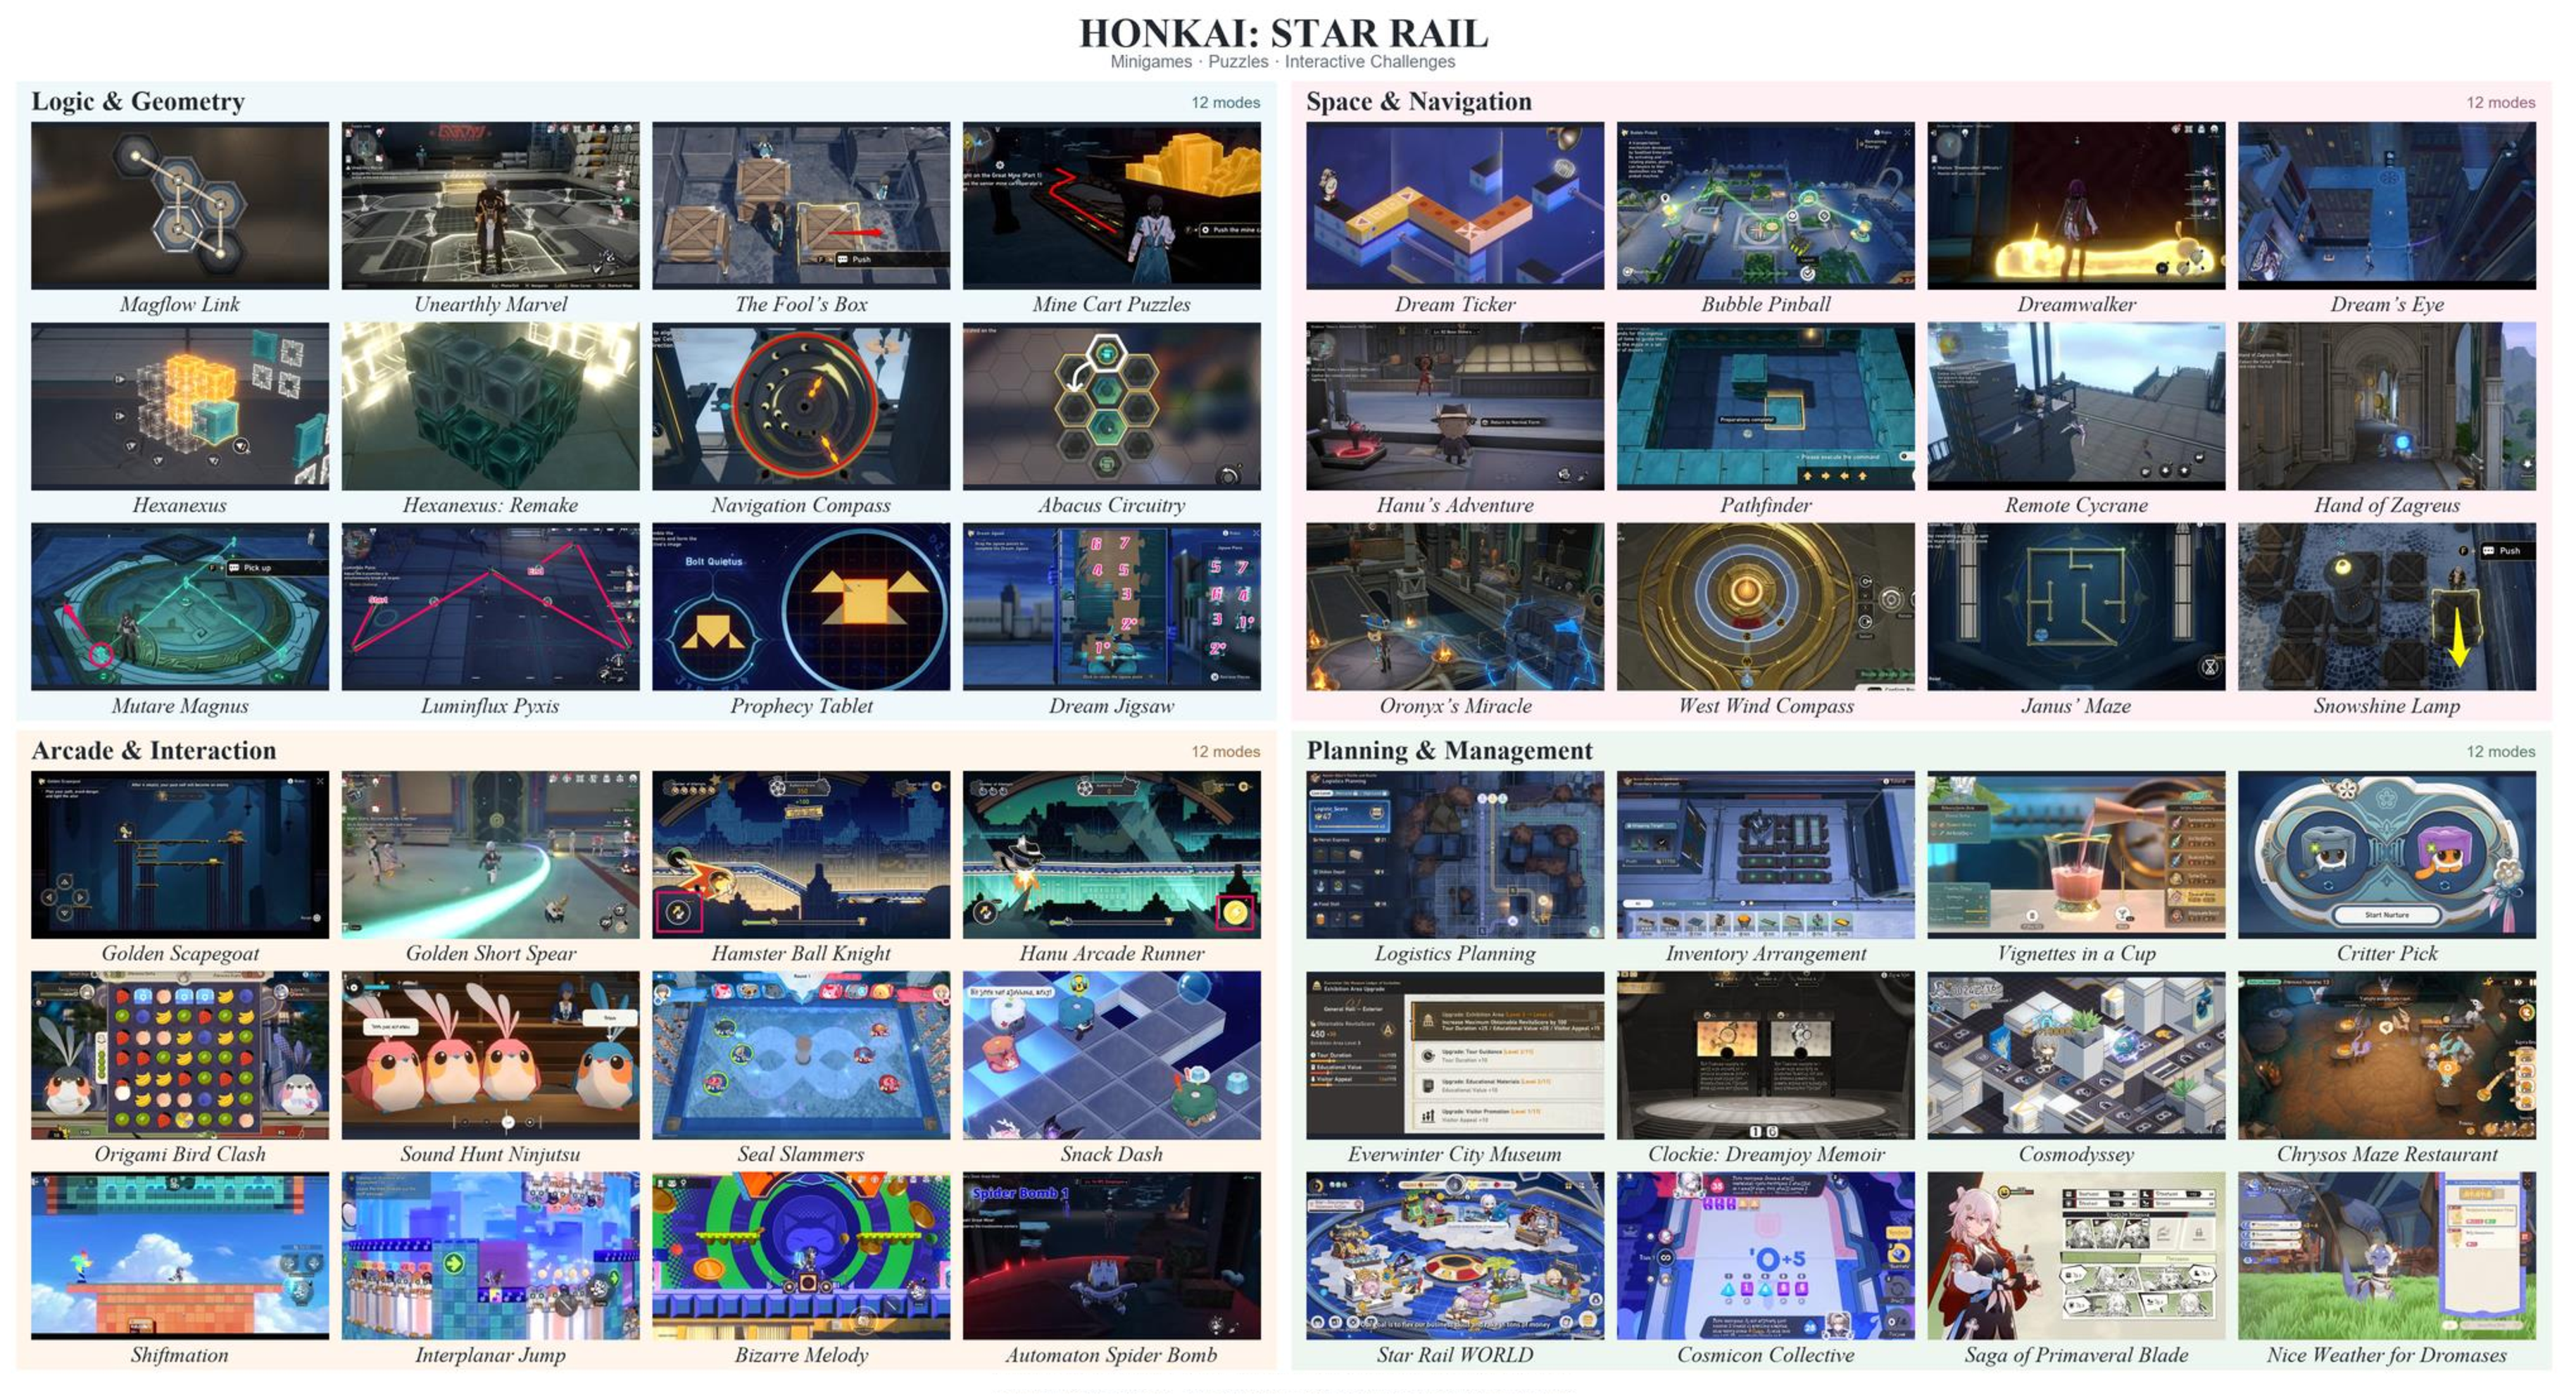
\includegraphics[width=\linewidth]{figs/hsr_minigame_all.pdf}
    \caption{
    \textbf{Representative minigames and interaction challenges in the Honkai: Star Rail evaluation suite.}
    This extended screenshot gallery illustrates the range of game interactions in Honkai: Star Rail. It is a qualitative visualization rather than the scored minigame inventory. The quantitative benchmark contains seven scored minigame types and 40 tasks, summarized in Figure~\ref{fig:hsr_minigames} and Table~\ref{tab:minigame_results}.
    }
    \label{fig:hsr_minigames_all}
\end{figure*}

\FloatBarrier

\section{Rollout Visualization and Qualitative Case Study}
\label{app:rl_rollouts}

The reward curves in Figure~\ref{fig:rl_reward} show how policy optimization progresses during training. To complement these aggregate measurements, we visualize how navigation and target interaction change across checkpoints. We compare the SFT initialization (CP 0) with five TA-GRPO checkpoints on a training task and a held-out development task. Each checkpoint is evaluated in 16 attempts from the same task and initial scene. The \textbf{Task successes} value on the left of each row reports the number of successful attempts, while twelve ordered frames depict one representative rollout. Executed actions and selected translated reasoning excerpts appear below the frames. The two views are complementary. The counts summarize reliability across attempts, and the screenshots make route selection, obstacle handling, and goal interaction easier to inspect.

\textbf{Training rollout: Reach Pom-Pom.} Figure~\ref{fig:rl_train_rollout} follows the policy through a multi-level interior with railings, corridors, and nearby interactable objects. The number of successful attempts grows from 3/16 for the SFT initialization to 14/16 at CP 20 and 15/16 at both CP 40 and CP 50. In the illustrated CP 20 rollout, the policy takes a route around the bar and completes the target interaction in 38.3 s. Later checkpoints also complete the displayed task. This case illustrates a useful progression from recognizing the destination to navigating the intervening geometry and executing the interaction that verifies completion. The visual examples and aggregated attempts together indicate more reliable goal-directed behavior after online training.

\begin{figure*}[!t]
    \centering
    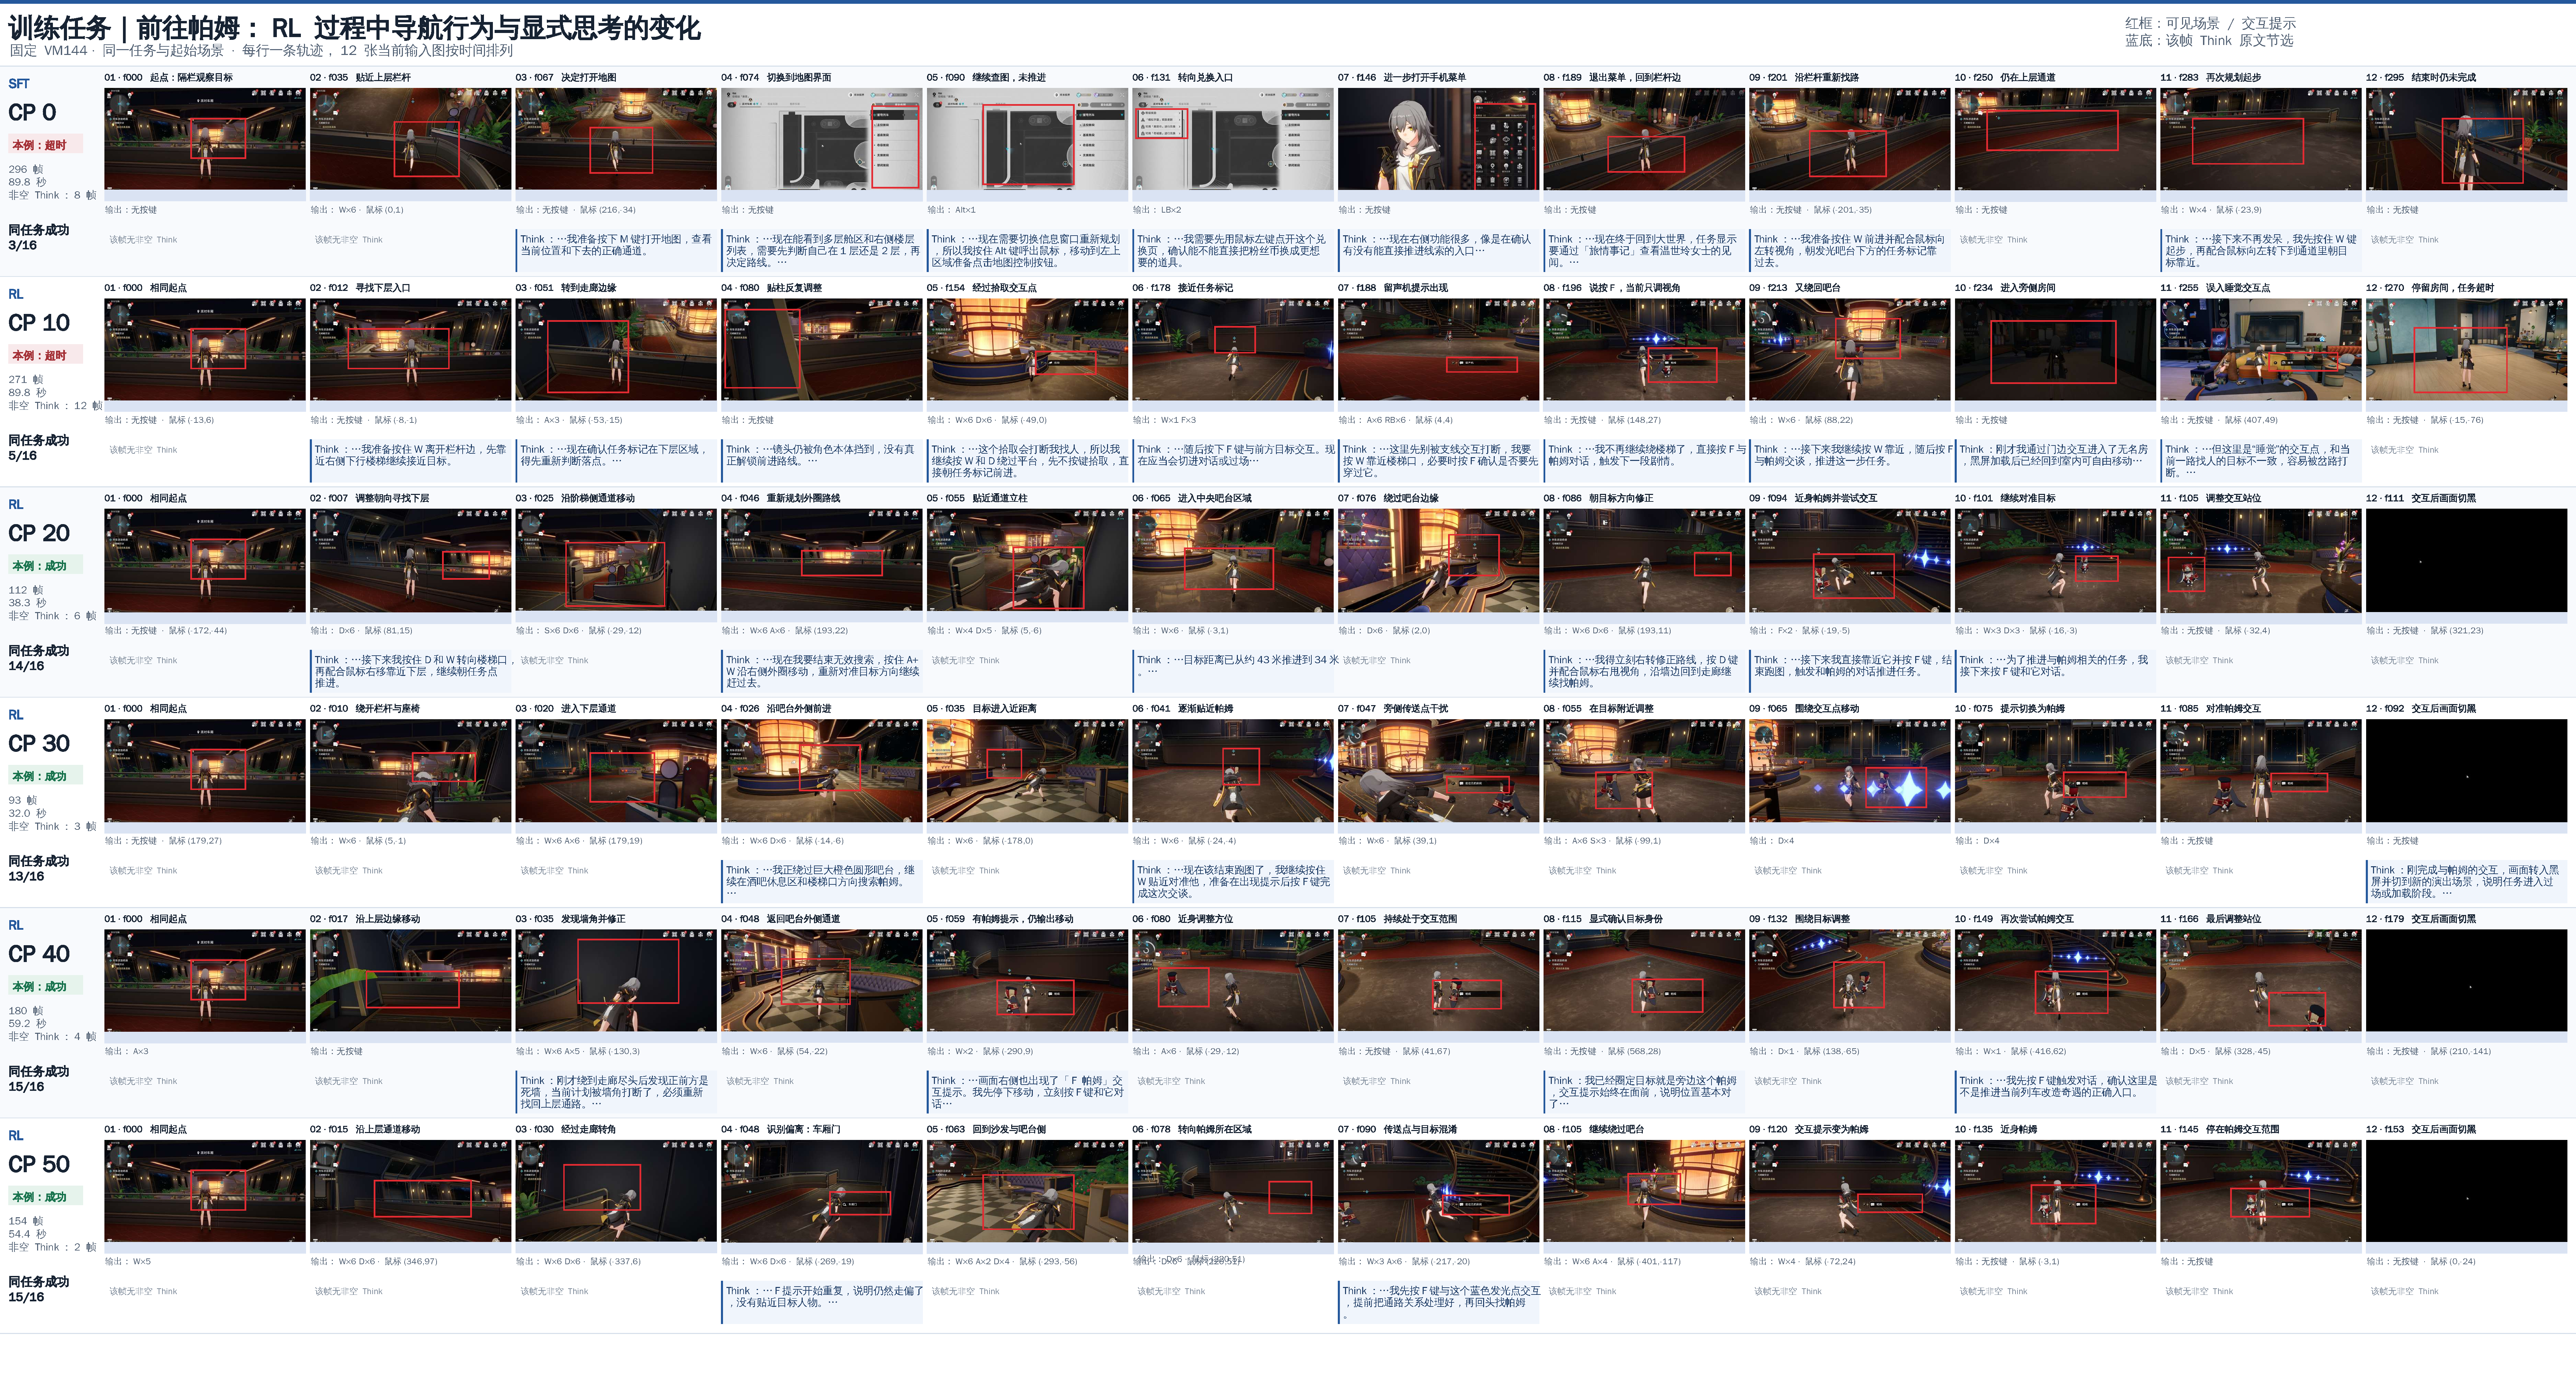
\includegraphics[width=0.98\textwidth]{figs/rl_train_rollout.pdf}
    \caption{\textbf{Navigation across RL checkpoints on a training task (Reach Pom-Pom).} Each row shows one representative rollout with twelve temporally ordered observations, actions, and translated reasoning excerpts. \textbf{Task successes} reports successful attempts out of 16 for each checkpoint: 3, 5, 14, 13, 15, and 15 for CP 0-50, respectively. Red boxes mark scene details or interaction prompts, and blue shading marks reasoning excerpts. The illustrated CP 0 and CP 10 attempts time out, while CP 20-50 reach the target and complete the interaction. Frame counts and completion times describe only the displayed rollout.}
    \label{fig:rl_train_rollout}
\end{figure*}

\textbf{Development rollout: Reach March 7th.} Figure~\ref{fig:rl_dev_rollout} examines whether similar behavior emerges on a held-out navigation objective. Successful attempts increase from 1/16 at the SFT initialization to 8/16 at CP 20 and 10/16 at CP 50. The illustrated CP 20 policy follows the lower street, navigates around a pillar, and initiates the required dialogue in 46.1\,s. CP 40 and CP 50 also complete the target interaction in their displayed rollouts. Because this task is not the RL training objective, the comparison provides complementary evidence that the learned navigation behavior can extend to a different destination and interaction sequence within the same game.

\begin{figure*}[!t]
    \centering
    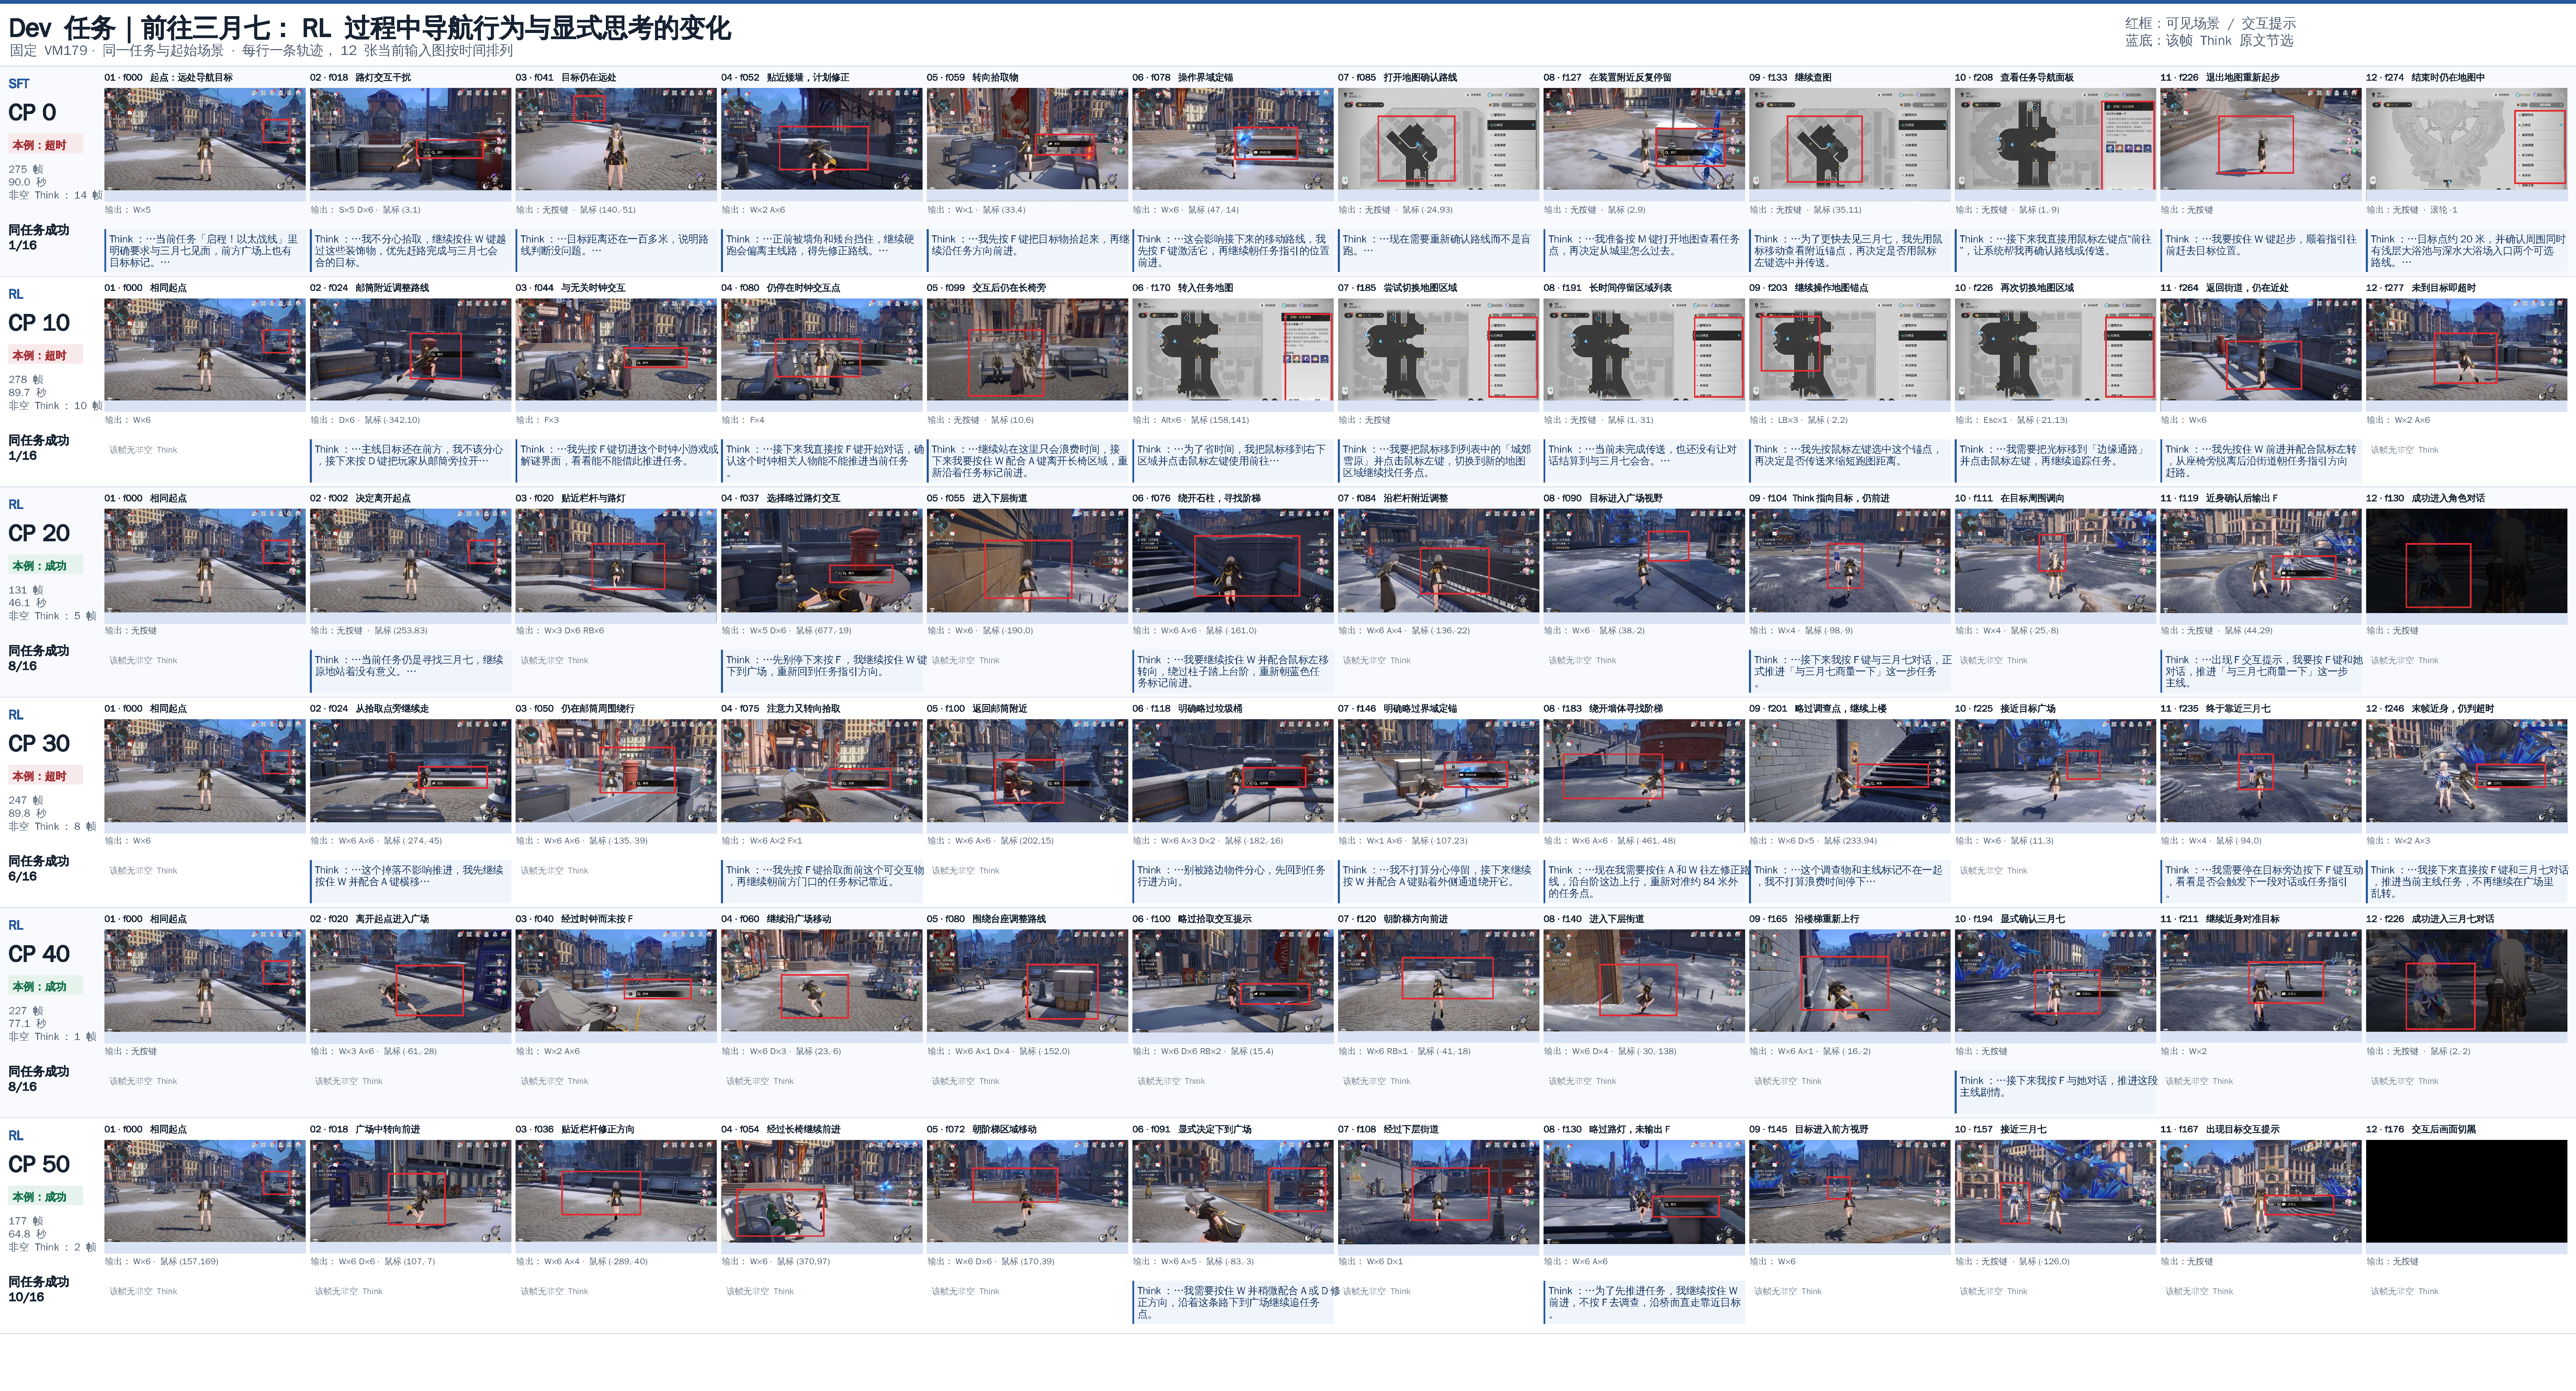
\includegraphics[width=0.98\textwidth]{figs/rl_dev_rollout.pdf}
    \caption{\textbf{Navigation across RL checkpoints on a development task (Reach March 7th).} Each row presents one representative rollout from the same task and initial scene, with twelve ordered observations, actions, and translated reasoning excerpts. \textbf{Task successes} counts successful attempts out of 16: 1, 1, 8, 6, 8, and 10 for CP 0-50, respectively. The illustrated CP 0, CP 10, and CP 30 attempts time out, whereas CP 20, CP 40, and CP 50 complete the target dialogue. Aggregate successes and representative trajectories provide complementary evidence of navigation and interaction progress.}
    \label{fig:rl_dev_rollout}
\end{figure*}

Across both cases, the increase in successful attempts is accompanied by more goal-directed behavior in the illustrated trajectories. Later policies more consistently select routes around obstacles, avoid unrelated interactions, and carry through to the final task-verifying action rather than stopping near the target location. The 16-attempt counts quantify the change in completion reliability, while the examples help interpret what that improvement looks like during execution. Together with the held-out side-quest results, they illustrate how online training can strengthen navigation and sustained goal pursuit.

\FloatBarrier

\section{Training Recipe and Reproducibility Details}
\label{app:training_recipe_details}

\subsection{Unified Verl-Based Training and Inference}
\label{app:unified_training_inference}

We extend Verl~\cite{sheng2024hybridflow} to use a shared game-interaction interface across CPT, SFT, and TA-GRPO. The training framework handles the stage-specific objectives and model updates, while Streaming-vLLM supplies autoregressive policy inference for interactive evaluation and online RL rollouts. The stages share the keyboard-mouse action grammar, observation-action history representation, and game-facing execution interface. CPT and SFT learn from recorded trajectories under their respective objectives, and TA-GRPO receives environment-verifiable feedback from interactions generated by the current policy. Consequently, the final policy is evaluated through the same type of executable control path used to collect online training experience.

\textbf{Consistency scope.} The system keeps action serialization, token boundaries, and environment timing consistent between training-stage evaluation and online policy interaction. It does not imply that every forward pass uses the same numerical kernel or cached context. Training computes gradients on supervised or rollout-derived sequences, whereas Streaming-vLLM uses stateful KV reuse, memory compaction, and architecture-dependent serving kernels. The RoPE phase adjustment in Appendix~\ref{app:rope_refresh} corrects retained cache positions but does not reconstruct the output of a fully re-encoded context. Consistency therefore refers to the policy interface and interaction semantics, not bitwise equality of training and inference logits.

\subsection{Training Configuration and Data Separation}

\textbf{Controlled CPT configurations.} The scaling study consists of four backbone sizes, five game mixtures, and six completed training budgets. It uses twenty primary Warmup-Stable-Decay (WSD) trunks, one per size-mixture pair. The shorter-budget checkpoints branch from their shared trunk and complete an independent decay phase within the stated total budget, yielding 120 evaluated configurations. All controlled runs use an 85\% gameplay and 15\% general vision-language token ratio, which is also retained for the separately trained HSR-augmented \ourmodel-CPT checkpoint. The CPT recipe uses BF16 AdamW with $\beta_1=0.9$, $\beta_2=0.95$, weight decay $0.01$, gradient clipping at $1.0$, and peak learning rates of $10^{-5}$ for the language model and $7\times10^{-6}$ for the unfrozen vision encoder. The WSD allocation is 3\% warmup, 87.3\% stable training, and 9.7\% cosine decay. The controlled grid uses 854$\times$480 observations, twenty visual turns per context, and approximately $2.3\times10^{5}$ supervised target tokens per update.

\textbf{Cross-stage implementation.} The same autoregressive device-level action representation is retained in CPT, SFT, and TA-GRPO, while instruction and memory conditioning are added in the later stages. The full stage-by-stage recipe, including the image resolution actually configured for each stage, is summarized in Table~\ref{tab:training_recipe}. For the real-time RL stage, the rollout-worker and training configuration are recorded separately from the controlled CPT grid. The short-term history uses 20 dialogue turns, the memory budget is 512 tokens, and each TA-GRPO segment is bounded by 20 dialogue turns with temporal factor $\beta=0.9$.

\textbf{Evaluation separation.} Training/validation/test splits are defined at the complete recording or task-source level before extracting overlapping action windows or multi-level examples. For interaction benchmarks, time-paused (TP) evaluation freezes the simulated environment during policy inference, whereas real-time (RT) evaluation lets the environment advance. These settings use the same action serialization but different timing semantics. Real-time performance comparisons should therefore report both the serving configuration and environment timing rather than treating model size or score as a proxy for latency.

\begin{table*}[t!]
\vspace{-6pt}
\begin{center}
\caption{
\textbf{Training recipes for \ourmodel.}
Stage I reports the controlled GameScaling reference on four Qwen3.5 Dense sizes. The HSR experiments use a separately trained \ourmodel-CPT checkpoint with additional \emph{Honkai: Star Rail} data and the same 85/15 gameplay-VLM token mixture, followed by SFT and TA-GRPO. RL run-dependent settings are reported for navigation (nav) and puzzle training (puzzle). RL token totals count generated response tokens, whereas supervised target tokens per update follow a different accounting convention.
}
\label{tab:training_recipe}

\resizebox{\linewidth}{!}{
\begin{tabular}{lccc}
& \texttt{Stage I} & \texttt{Stage II} & \texttt{Stage III} \\
\toprule[0.95pt]
Phase & CPT & SFT & RL \\

\midrule[0.6pt]
\multicolumn{4}{c}{\textbf{Model and Context Configuration}} \\
\midrule[0.6pt]
\textbf{Qwen3-VL (supported)} & \multicolumn{3}{c}{Dense: 2B, 4B, 8B, 32B, MoE: 30B-A3B} \\
\textbf{Qwen3.5 (supported)} & \multicolumn{3}{c}{Dense: 0.8B, 2B, 9B, 27B, MoE: 35B-A3B} \\
Controlled CPT Scales & 0.8B / 2B / 9B / 27B & -- & -- \\
Image Resolution & $854\times480$ & $854\times480$ & $854\times480$ \\
Visual Observation Rate & 5 Hz & 5 Hz & 5 Hz \\
Low-Level Control Rate & 30 Hz & 30 Hz & 30 Hz \\
Local Visual History & 20 observation turns & 20 observation turns & 20 observation turns \\
Maximum Context Length & 45K & 45K & 23K \\
Short-Term History Budget $L_H$ & -- & 20 dialogue turns & 20 dialogue turns \\
Long-Term Memory Budget $L_M$ & -- & 512 tokens & 512 tokens \\

\midrule[0.6pt]
\multicolumn{4}{c}{\textbf{Training Hyper-Parameters}} \\
\midrule[0.6pt]
Initialization & Base & CPT & SFT \\
Optimizer & AdamW & AdamW & Adam (MCore) \\
Optimizer Hyper-Parameters & $\beta_1,\beta_2=0.9,0.95$ & $\beta_1,\beta_2=0.9,0.95$ & $\beta_1,\beta_2=0.9,0.999$ \\
\multirow{2}{*}{Learning Rate}
& $1\times10^{-5}$ (LLM) & $1\times10^{-5}$ (LLM) & $1\times10^{-6}$ (LLM) \\
& $7\times10^{-6}$ (vision encoder) & $1\times10^{-5}$ (vision encoder) & $1\times10^{-6}$ (vision encoder) \\
Weight Decay & 0.01 & 0.1 & 0.01 \\
Gradient Clipping & 1.0 & 1.0 & 1.0 \\
Training Precision & BF16 & BF16 & BF16 \\
Learning Rate Scheduler & Warmup-Stable-Decay & Warmup-Decay & Constant \\
Warmup / Stable / Decay & 3\% / 87.3\% / 9.7\% & 5\% / -- / 95\% & 0\% / 100\% / 0\% \\
Minimum LR Ratio & 0.1 & 0.1 & -- (constant LR) \\
Global Supervised Tokens / Update & $2.3\times10^{5}$ & $2.3\times10^{5}$ & -- \\
Training Iterations & 6,839 & 1,696 & 61 (nav) / 53 (puzzle) \\
Optimizer Updates & -- & -- & 122 (nav) / 106 (puzzle) \\
Total Training Tokens & $5.45\times10^{10}$ & $3.9\times10^{8}$ & $3.1\times10^{7}$ (nav) / $2.8\times10^{7}$ (puzzle) \\

\midrule[0.6pt]
\multicolumn{4}{c}{\textbf{Stage-Specific Configuration}} \\
\midrule[0.6pt]
Random Key Remapping & \checkmark & -- & -- \\
Repeat Decay $\gamma$ & 0.9 & -- & -- \\
Multi-level Supervision & -- & \checkmark & \checkmark \\
Cross-Context Memory & -- & \checkmark & \checkmark \\
Parallel Environments & -- & -- & 32 Windows VMs \\
Inference Services & -- & -- & Sharded pool (64 H200) \\
Tasks per Iteration & -- & -- & 8 (nav) / 16 (puzzle) \\
Rollouts per Iteration & -- & -- & 128 \\
Rollouts per Task & -- & -- & 16 (nav) / 8 (puzzle) \\
Group Size $G$ & -- & -- & 8 \\
Maximum Segment Length & -- & -- & 20 dialogue turns \\
Temporal Factor $\beta$ & -- & -- & 0.9 \\
Policy Clip $\epsilon_{\mathrm{clip}}$ & -- & -- & 0.2 \\
Updates per Rollout Batch & -- & -- & 2 (disjoint half-batches) \\

\midrule[0.6pt]
\multicolumn{4}{c}{\textbf{Training Data}} \\
\midrule[0.6pt]
Primary Data & Cross-Game $+$ General VLM & Multi-Level HSR & Online Interaction \\
Supervision & Actions & Reasoning + actions & Verifiable binary task rewards \\
Data Size & $\sim$2.4K h & $\sim$1K h (annotated pool) & $\sim$7.8K (nav) / $\sim$6.8K (puzzle) rollouts \\
\bottomrule[0.95pt]
\end{tabular}
}
\end{center}
\vspace{-4pt}
\end{table*}

\subsection{Execution Protocol and Reproducibility}
\label{app:runtime_manifest}

\textbf{Rollout and evaluation protocol.}
Interactive inference produces six keyboard-mouse control blocks from the current visual observation, task instruction, and memory context. The client executes these blocks while the environment continues to advance. Online RL runs across 32 parallel game environments served by a sharded Streaming-vLLM pool with 64 NVIDIA H200 GPUs. Each iteration gathers 128 rollouts in groups of eight from the active navigation or puzzle task pool. Two disjoint rollout subsets support the policy updates, and environment task verification provides rewards without a learned process reward model. SFT and RL evaluations use matched task initializations, milestone verifiers, action semantics, and inference settings as described in Sec.~\ref{sec:exp_rl}.

\textbf{Reproducibility boundary.}
After the two policy updates, the resulting checkpoint is synchronized across the inference services, and the next rollout iteration starts only after the workers acknowledge the expected policy version. Our run audit records the trainer and inference revisions, checkpoints, action serialization, tokenizer, image preprocessing, and environment settings. Inference uses BF16 with a maximum generation length of 512 tokens and temperature 0.9. The game screenshots are captured at $1280\times720$ and resized to $854\times480$ for model input. TA-GRPO uses 20-turn segments and temporal factor $\beta=0.9$. These settings, together with the checkpoint and service synchronization protocol, specify the interaction conditions used in the reported experiments.




